% Main document of the project, this will include all the other parts involving the documentation...

\documentclass[a4paper]{article}
\usepackage[utf8]{inputenc}
\usepackage[T1]{fontenc}

%% Sets page size and margins
\usepackage[a4paper,top=3cm,bottom=2cm,left=3cm,right=3cm,marginparwidth=1.75cm]{geometry}

%% Useful packages
\usepackage[table,xcdraw]{xcolor}
\usepackage{longtable}
\usepackage{amsmath}
\usepackage{floatrow}
\usepackage{graphicx}
\graphicspath{ {./images/} }
\usepackage[colorinlistoftodos]{todonotes}
\usepackage[colorlinks=true, allcolors=blue]{hyperref}
\usepackage{amsmath}
\usepackage{chngcntr}
\usepackage{wrapfig}
\usepackage{eurosym}
\usepackage{caption}
\usepackage{subcaption}
\usepackage{listings}
\usepackage{placeins}
\usepackage{multicol}
\usepackage{verbatim}
\usepackage{csvsimple}
\usepackage{listings}
\usepackage[spanish]{babel}
\renewcommand\spanishtablename{Tabla}
\selectlanguage{spanish}
\usepackage{colortbl}
\usepackage{cite}
\usepackage{xr}

\usepackage[toc,page]{appendix}
\usepackage{pdflscape}

\expandafter\def\expandafter\appendixpagename%
\expandafter{\expandafter\Huge\appendixpagename}

\usepackage{afterpage}

\addto\captionsspanish{%
  \renewcommand\appendixname{\Huge Apéndices}
  \renewcommand\appendixpagename{\Huge Apéndices}
}

\captionsetup[table]{position=bottom}

\renewcommand{\lstlistingname}{Código}% 
\renewcommand{\lstlistlistingname}{Lista de código}% List of Listings -> List of Algorithms

% extracted from internet: https://timmurphy.org/2014/01/27/displaying-code-in-latex-documents/
\definecolor{lbcolor}{rgb}{0.93,0.93,0.93}
\lstset{  
    frame=tb, % draw a frame at the top and bottom of the code block
    tabsize=4, % tab space width
    showstringspaces=false, % don't mark spaces in strings
    numbers=left, % display line numbers on the left
    commentstyle=\color{green}, % comment color
    keywordstyle=\color{blue}, % keyword color
    stringstyle=\color{red},
    %backgroundcolor=\color{lbcolor}
}

\definecolor{main-color}{rgb}{0.6627, 0.7176, 0.7764}
\definecolor{back-color}{rgb}{0.1686, 0.1686, 0.1686}
\definecolor{string-color}{rgb}{0.3333, 0.5254, 0.345}
\definecolor{key-color}{rgb}{0.8, 0.47, 0.196}

\lstdefinestyle{idlstyle}
{
    language = C++,
    keywordstyle = {\color{key-color}},
    keywordstyle = [3]{\color{blue}},
    otherkeywords = {in, int ,interface, out, inout},
    morekeywords = [3]{in, out, inout}
}

\lstdefinestyle{JStyle}{
	numberbychapter=false,
	backgroundcolor=\color{white},   
	commentstyle=\color{teal},
	% 	keywordstyle=\,
	% numberstyle=\tiny\color{mGray},
	% 	stringstyle=\color{red},
	% 	basicstyle=\scriptsize,
	basicstyle=\small,
	breakatwhitespace=false,         
	breaklines=true,                 
	captionpos=b,                    
	keepspaces=true,                 
	numbers=left,                    
	numbersep=3pt,                  
	showspaces=false,                
	showstringspaces=false,
	showtabs=false,                  
	tabsize=2,
	language=C++,
	frame=lines,
	classoffset=1,
	morekeywords={\#pragma, omp, oss, parallel, single, taskwait, task, depend, firstprivate, priority},keywordstyle=\color{blue}\bfseries,
	otherkeywords = {\#pragma, omp, oss, parallel, single, taskwait, task, depend, firstprivate, priority}
}

\setcounter{secnumdepth}{3}
\setcounter{tocdepth}{3}

% \title{Integrating COMPSs and OmpSs Programming Models to support distributed heterogeneous computing environments}
\title{Integrating COMPSs and OmpSs Programming Models to support distributed heterogeneous computing environments}
\author
{
Marc Domínguez de la Rocha
\and
Rosa M. Badia
\and
Jorge Ejarque
}

\date{Junio 2019}

\begin{document}

\maketitle

\newpage
\renewcommand{\contentsname}{Índice}
\tableofcontents
\newpage

%GEP

La sección que continúa es relativa a la gestión del proyecto y se mantiene dentro del trabajo porque corresponde al estado del arte. El resto de secciones que conforman la gestión del proyecto se encuentran en los apéndices \ref{sec:sostenibilidad} \ref{sec:planificacion}

% La siguiente seccion enmarca el contexto
% que envuelve al proyecto y de alguna
% manera el por qué
\section{Contexto}

Hoy en día se tiende a tener distintos recursos de cómputo en un solo dispositivo, por ejemplo, en un teléfono móvil ya tenemos al menos un procesador y una tarjeta gráfica, pero no tan sólo en el ámbito más cotidiano (aunque no nos demos cuenta), sino que en los más profesionales y especializados está siendo también cada vez más común la heterogeneidad de los recursos de computación. 
\par\bigskip

El proyecto pretende facilitar la gestión de estos recursos de computación en entornos distribuidos, brindando un método robusto y eficiente para programar aplicaciones en estos entornos.
%Quienes son los actores? Quien se beneficia?


\subsection{Introducción}

Este proyecto es un Trabajo de Fin de Grado del Grado en Ingeniería Informática, especializado en el área de Ingeniería de Computadores. El grado es impartido por la \textit{Facultat d'Informàtica de Barcelona (FIB)} centro perteneciente a la \textit{Universitat Politècnica de Catalunya (UPC)}. 
\par\bigskip

El proyecto se desarrollará conjuntamente con el \textit{Barcelona Supercomputing Center (BSC)}, estudiaremos como podemos integrar los modelos de programación \textit{COMPSs} y \textit{OmpSs} para alcanzar este objetivo, implementaremos un prototipo y evaluaremos su rendimiento y características deseadas. 
%Indagar en cuales son estas caracteristicas? 

\subsection{Actores}

Los actores en este proyecto serán las personas que tomen parte en él, ya sea de manera directa o indirecta. Con esto quiero decir, que tanto las personas que tomen parte en el desarrollo \textit{per se} como las personas que se nutran de este, serán los actores.

\begin{itemize}
 \item \textbf{Desarrollador:} La figura del desarrollador \textbf{debe} ser la persona que trabaje de manera más directa en el proyecto. En este proyecto únicamente habrá un desarrollador que ha elaborado la documentación que leerás a continuación y dará forma a los objetivos tangibles del proyecto.  
 \item \textbf{Director y codirector:} Pese a que el desarrollador tendrá el papel principal en el proyecto, el director y el codirector le guiarán en el camino abierto que es el desarrollo del proyecto. Se establecerán reuniones de seguimiento donde serán capaces de hacer un correcto supervisamiento de las actividades propuestas para el proyecto.
 \item \textbf{Barcelona Supercomputing Center:} De manera directa el centro otorga al desarrollador un lugar de trabajo y un equipo informático. Por otra parte, cuenta con el soporte por parte de los equipos de desarrollo de \textit{COMPSs} (del cual forma parte el desarrollador) y de \textit{OmpSs} para cualquier incidencia relacionada con su \textit{software} y derivados.
 \item \textbf{Beneficiarios:} \textit{COMPSs} es utilizado para proyectos europeos en los cuales el \textit{BSC} toma parte, el proyecto podrá ser útil para algunos de ellos, además todo departamento del \textit{BSC} que utilice \textit{COMPSs} para el desarrollo de aplicaciones podrá utilizarlo.
\end{itemize}

\section{Estado del arte}

%check si te estas patillando lo de ``centenares''
Existen centenares de modelos de programación, véanse \textit{OpenMP}, \textit{OmpSs}, \textit{MPI}, \textit{COMPSs} y un largo etcétera. De alguna manera el objetivo en común fue y es aprovechar los cada vez más abundantes recursos en las máquinas, que finalmente no sólo han crecido en abundancia si no en diversidad. La filosofía sigue siendo la misma, sacar el mayor rendimiento posible a nuestras máquinas. 
\par\bigskip

Para esto son necesarios modelos de programación que nos den la posibilidad de utilizar los recursos y nos ayuden a explotar la posible sinergia entre estos en ciertas aplicaciones. 
\par\bigskip

La diferencia más elemental entre los modelos, es en como se gestiona la memoria, o bien como la memoria está dispuesta en el modelo. Con \textit{shared memory} (\textit{OpenMP}, \textit{OmpSs}...), se aprovecha que el conjunto de hilos de ejecución (\textit{threads}) comparten la memoria, con \textit{distributed memory} (\textit{MPI}...) que se utilizan diferentes procesos con la posibilidad de que estos estén distribuidos entre distintos nodos, existen también modelos como \textit{CUDA} y \textit{OpenCL} que transfieren memoria de la \textit{CPU} a la memoria del acelerador en cuestión.
\par\bigskip

La integración de los modelos propuestos \textit{COMPSs} y \textit{OmpSs} nos otorgará la posibilidad de utilizar todos los recursos de la máquina, a continuación se ahonda en las características de ambos.

\subsection{COMPSs}

\textit{COMPSs} es desarrollado por el grupo \textit{Workflows and Distributed Computing} que pertenece al departamento de \textit{CS - Computer Science}.
\par\bigskip

\textit{COMPSs} es un modelo de programación para entornos distribuidos basado en la generación de tareas, el objetivo es hacer más sencilla la programación de aplicaciones y su ejecución en entornos distribuidos (clústers y \textit{clouds}, por ejemplo)\cite{badia2015comp}.La generación de tareas la efectua un programa principal ejecutado en secuencial, las tareas se especifican mediante la anotación de las funciones que se deseen, en tiempo de ejecución se genera un grafo de tareas y se detectan las dependencias entre estas para ejecutarlas en el orden correcto. Dado que está preparado para ejecutarse en entornos distribuidos también se detecta cuando son necesarias transferencias entre nodos.   \par\bigskip

Para facilitar más aún el uso del modelo, está dotado de un sistema de \textit{runtime} compuesto por un \textit{master} y un conjunto de \textit{workers}, el \textit{runtime} coexiste con la aplicación. Se encarga de detectar las dependencias que puedan surgir entre las tareas que genera el programa principal y las ejecuta a medida que las dependencias se resuelven. 
%\par\bigskip

\subsubsection{Modelo de programación} 
\label{compss_pm}

El \textit{runtime} de \textit{COMPSs} está implementado en \textit{Java} por lo cuál se soporta dicho lenguaje, además se desarrollaron los \textit{bindings} de \textit{Python}\cite{tejedor2017pycompss} y \textit{C/C++} para facilitar el portaje de aplicaciones en estos lenguajes a \textit{COMPSs}. 
\par\bigskip

Dicho esto, centraremos nuestros esfuerzos en \textit{C} y \textit{C++}. Para desarrollar una aplicación de \textit{COMPSs} en \textit{C/C++} necesitamos el programa principal (ejecutado en secuencial), una interfaz que especificará las funciones que \textit{a posteriori} serán tareas, y el código que realmente implementan estas tareas. 
\par\bigskip

Veamos en orden de enumeración ejemplos de los componentes de una aplicación.

%EJEMPLO INTERFACE
\begin{lstlisting}[caption={Interfaz de la aplicación 'ejemplo'.},captionpos=b, label={lst:ejemplo.idl}, style=idlstyle]
interface ejemplo {
    void funcionEjemplo(in int a, out int[a] array_a);
};
\end{lstlisting}

La interfaz de la imagen superior define una función llamada funcionEjemplo con un parámetro de entrada y uno de salida, las palabras clave \textit{in} y \textit{out} respectivamente otorgan estas propiedades a los parámetros, también se puede combinar con \textit{inout}. Cualquier llamada a la función será ejecutada como tarea.\smallskip

%EJEMPLO MASTER CODE
\begin{lstlisting}[caption={Fracción del código del programa principal}, captionpos=b, label={lst:ejemplo.cc}, language=C++]
    compss_on();

    int a = 10;
    int* array_a;

    funcionEjemplo(a, array_a);

    compss_wait_on(array_a);

    compss_off();
\end{lstlisting}

Esta imagen muestra el código del programa principal de manera reducida. Es tan sencillo como prometía, encendemos el \textit{runtime} de \textit{COMPSs}, preparamos los parámetros de la función, ejecutamos y finalmente esperamos a los parámetros de salida y apagamos el \textit{runtime}. \smallskip

\begin{lstlisting}[caption={Implementación de la función 'funcionEjemplo'}, captionpos=b, label={lst:ejemplo-functions.cc}, language=C++]
void funcionEjemplo(int a, int array_a[]) {
    for (int i = 0; i < a; ++i) {
        array_a[i] = a;
    }
}
\end{lstlisting}

Las tareas se implementan como funciones que serán ejecutadas por los workers. Salvo convenciones en los nombres de los ficheros para hacer la compilación de la aplicación esto es todo lo necesario para desarrollar una aplicación en \textit{COMPSs} de \textit{C/C++}.

\begin{comment}
\subsubsection{Compilación}

Para compilar la aplicacion en \textit{COMPSs} de \textit{C/C++}, 

\begin{figure}[H]
    \centering
    \caption{Proceso de compilado de una aplicación COMPSs C/C++}
%    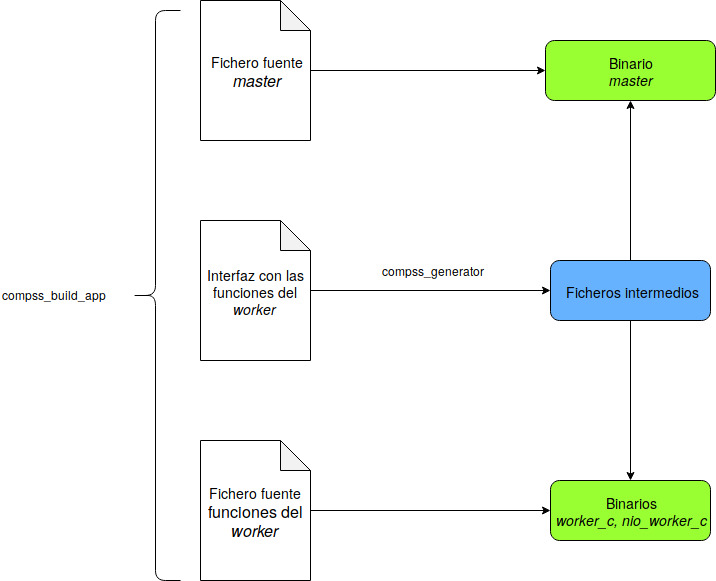
\includegraphics[width=\textwidth]{proceso_compilado.jpg}
    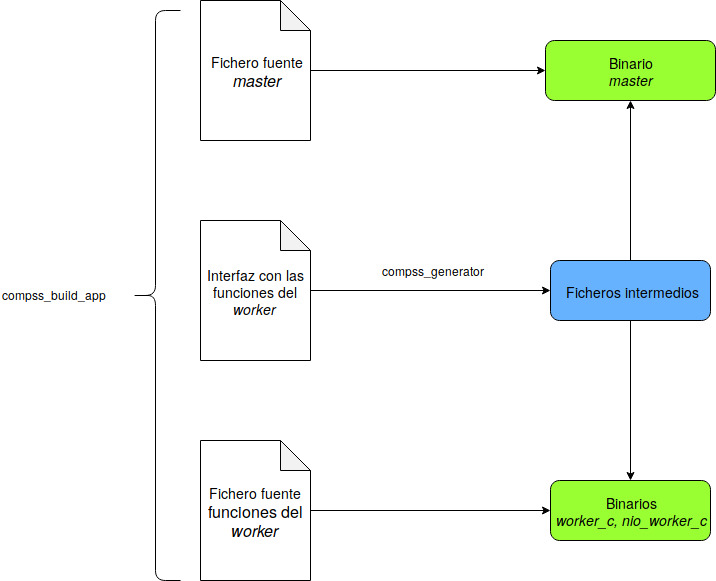
\includegraphics[scale=0.5]{proceso_compilado.jpg}
    \label{fig:proceso_compilado}
\end{figure}
\end{comment}

\subsubsection{Modelo de ejecución\label{modeloejecucion}}

El modelo de ejecución es sencillo, muy similar al modelo \textit{thread-pool}, al iniciar el \textit{runtime} se levanta el \textit{master} y un conjunto de \textit{workers}, a medida que se vayan generando tareas se estudiará qué \textit{workers} están libres y si cumplen los requisitos para ejecutar dicha tarea, y en ese caso la ejecutarán. 

\begin{figure}[H]
    \centering 
    \caption{Modelo de ejecución, basado en la aplicación 'ejemplo'.}
    %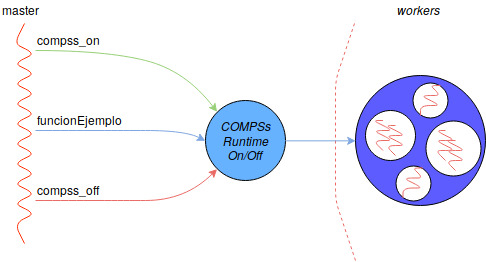
\includegraphics[width=\textwidth]{sta-masterworker.jpg}
    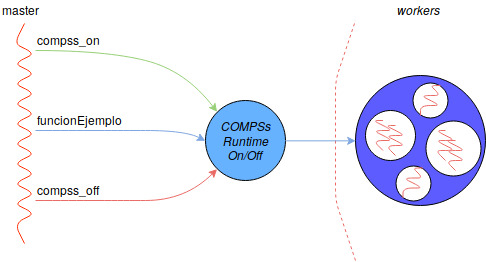
\includegraphics[scale=0.75]{sta-masterworker.jpg}
    \label{fig:masterworker_pool}
\end{figure}

La imagen muestra lo que sucede al ejecutar la aplicación de ejemplo de la sección \ref{compss_pm}, las líneas rojas curvas indican procesos (o bien \textit{threads}), lo importante sucede entre las flechas etiquetadas como compss\_on y compss\_off, la ejecución de la tarea. Se pide ejecutar la tarea funcionEjemplo al \textit{runtime} de \textit{COMPSs} y se decide en qué \textit{worker} se ejecutará. Hasta aquí podríamos pensar que es indéntico al \textit{thread-pool}. Nótese, que esto no es así, por el hecho de que no tenemos por qué hablar de una misma máquina, sino que pueden ser máquinas distintas, como se puede ver en el grupo de ordenadores de la imagen. 
\par\bigskip

En \textit{C/C++} existen dos tipos de \textit{worker}, uno \textbf{no persistente} y otro \textbf{persistente}. 

\begin{itemize}
 \item \textbf{No persistente:} Para cada tarea que se quiere ejecutar en uno de estos workers se debe crear el \textit{thread} y unas \textit{pipes} para hacer \textit{Inter-process communication} (IPC). %No sé si indagar en qué se pasa por las pipes, hmmm... qué se pasa por las pipes?
 \item \textbf{Persistente:} Este tipo de \textit{worker} se levanta una vez al inicio de la aplicación y espera recibir las tareas a ejecutar.
\end{itemize}


\subsection{OmpSs}

\textit{OmpSs} es desarrollado por el grupo \textit{PM - Programming Models}, perteneciente también al departamento de \textit{CS - Computer Science}.
\par\bigskip

\textit{OmpSs} es un modelo de programación que intenta explotar el paralelismo de las aplicaciones de una manera sencilla y aprovechando al máximo los recursos de la máquina\cite{duran2011ompss}. 
\par\bigskip
El nombre del modelo proviene de \textit{OpenMP} y \textit{StarSs} (modelo que desarrolló el \textit{BSC}), este integra funcionalidades presentes en ambos. Por parte de \textit{OpenMP} se quiere tomar la facilidad de paralelizar una aplicación secuencial insertando pragmas, y de \textit{StarSs} el modelo de ejecución basado en un \textit{thread-pool} y que permite la ejecución de código en más recursos que únicamente el procesador, es decir, que ofrece fácil gestión del resto de recursos de cómputo (\textit{GPUs}, \textit{FPGAs}, ...)\cite{sainz2014leveraging}\cite{filgueras2013heterogeneous}.

\subsubsection{Modelo de programación y ejecución}

El modelo de programación de \textit{OmpSs} se basa en la generación de tareas sencillamente insertando pragmas en código secuencial y a su vez facilitando la gestión de recursos heterogéneos. Veamos un pequeño ejemplo que muestre estas facultades.

\begin{lstlisting}[caption={Multiplicación de un bloque de una matriz utilizando GPUs.}, captionpos=b, label={lst:ompssmatmul.cc}, style=JStyle]
for (int i = 0; i < N; ++i) {
    for (int j = 0; j < N; ++j) {
        for (int k = 0; k < N; ++k) {
            #pragma omp target device(cuda) \
                               copy_deps    \
                               ndrange(2,N,N,32,32)
            #pragma omp task inout([N*N]C) in([N*N]A, [N*N]B)
            multiply_partitions_GPU(A[i*N+k], 
                                    B[k*N+j], 
                                    C[i*N+j], 
                                    n);
        }
    }
}
\end{lstlisting}

El código muestra una multiplicación de matrices por bloques. Con el primer pragma se indica que el dispositivo objetivo es una tarjeta gráfica que soporte \textit{CUDA}, y el segundo la declaración de una tarea y el tamaño de los bloques junto a las dependencias de esta.
\par\bigskip

El modelo de ejecución consiste en un \textit{thread-pool}, es decir, al generar tareas se escogerán \textit{threads} del \textit{pool} (entendámoslo como un conjunto de \textit{threads}) para ejecutarlas.
\par\bigskip

Cabe decir que para compilar una aplicación de \textit{OmpSs}, se utiliza el compilador \textit{source-to-source Mercurium} y el runtime \textit{Nanos++} para gestionar el paralelismo, es decir, la creación de tareas, sincronización entre estas, etc.

\subsection{COMPSs+OmpSs} 
\label{sec:compssompss}

Actualmente existe la posibilidad de desarrollar aplicaciones que utilicen \textit{OmpSs} dentro de \textit{COMPSs}. 
\par\bigskip
Para poder interactuar con el \textit{runtime} de \textit{OmpSs} \textit{Nanos++}, necesitamos gestionarlo nosotros manualmente o bien utilizar los pragmas que nos propone el modelo de programación y compilar con \textit{Mercurium}. Entonces, asegurándonos de registrar los \textit{workers} en el \textit{runtime} y compilando su código fuente con \textit{Mercurium} aseguramos la interacción con el \textit{runtime} y por lo tanto la integración de ambos modelos.

Es posible desarrollar aplicaciones, como ya se ha comentado, pero con ciertas restricciones. Las problemáticas aparecen con los dos tipos de \textit{worker} que hemos visto antes. Para el worker no persistente, no suele valer la pena debido a la granularidad de las tareas de \textit{OmpSs}. El \textit{overhead} proviene de crear el \textit{thread} del \textit{worker}, registrarlo en el \textit{runtime Nanos++} y levantar las \textit{pipes}. El persistente carece del \textit{overhead} de levantar las \textit{pipes} y el resto, vale la pena ya que el \textit{worker} persiste durante la ejecución de la aplicación. Pese a que el persistente mejora respecto al no persitente, hay problemas de migración de \textit{threads} entre aplicaciones cuando se ejecutan varias a la vez.
\par\bigskip

Estos problemas pretenden arreglarse integrando \textit{OmpSs-2}, que ofrece un \textit{runtime} nuevo llamado \textit{Nanos6} y nuevas características que vienen con este cambio como por ejemplo:

\begin{itemize}
\item \textbf{Liberación de las dependencias:} Las dependencias en esta versión se liberen de manera temprana, es decir, una vez una tarea acaba con un dato lo notifica al \textit{runtime} y este se encarga de notificar a las tareas que quedan libres de esta dependencia.
 \item \textbf{Relajación de las dependencias:} Ahora se pueden utilizar nuevos pragmas para determinar dependencias más suaves, no tan estrictas como en la versión anterior.
 \item \textbf{Ejecución de funciones de manera asíncrona:} La \textit{API} del nuevo \textit{runtime} \textit{Nanos6} permite ejecutar de manera asíncrona funciones en forma de tarea a partir de un puntero a una función.
\end{itemize}

Hemos listado las que de alguna manera eran clave para el proyecto, \textit{OmpSs-2} implementa muchas otras mejorías a parte de estas\cite{OmpSs2reference}. Una vez integrado, el proyecto estudiará si realmente han sido solucionadas las problemáticas anteriormente planteadas.

\section{Alcance del proyecto}

En esta sección se declaran las intenciones del proyecto (qué se pretende hacer), mediante una serie de requerimientos que harán que el proyecto pueda ser acabado con éxito, y unos objetivos que marcarán el desarrollo de este. También los posibles riesgos que surjan (y las soluciones de estos) y la metodología de trabajo que se llevará a cabo.

\subsection{Requerimientos}

 Los requerimientos necesarios para este proyecto son:

\begin{itemize}
 \item La nueva integración con \textit{OmpSs-2} no debe romper la actual compatibilidad con \textit{OmpSs}.
 \item El rendimiento de las aplicaciones desarrolladas con \textit{COMPSs+OmpSs-2} debe mejorar.
 \item Todas las modificaciones sobre \textit{COMPSs} deben ajustarse al grupo de \textit{Workflows and Distributed Computing}.
 \item Cualquier requerimiento impuesto (o aconsejado) por el \textit{BSC} formará parte de esta lista.
  
\end{itemize}

\subsection{Objetivos}

El objetivo principal de este proyecto es reformular la integración de \textit{COMPSs} con \textit{OmpSs} para solucionar los problemas actuales, ya sea integrándolo de nuevo pero esta vez con \textit{OmpSs-2} o bien idear otra manera de resolver las problemáticas. La siguiente lista muestra la posible descomposición de objetivos:

\begin{itemize}
  \item Aprender a utilizar la API (\textit{Application Programming Interface}) de \textit{Nanos6}.
  \item Eliminar o bien reducir las problemáticas planteadas en la sección   \ref{sec:compssompss}.
  \item Mejorar la gestión de recursos heterogéneos en las aplicaciones desarrolladas en \textit{COMPSs} integrando \textit{OmpSs-2}.
  \item En caso de conseguir el resto de objetivos plantear la integración en \textit{Java} y \textit{Python}.
\end{itemize}

\subsection{Riesgos}

Durante el desarrollo del proyecto pueden surgir problemas, para mejorar la reacción ante ellos listaremos los posibles riesgos y las respectivas soluciones.

\subsubsection{Problemas con el material de desarrollo}

Se podría romper el equipo en el cual se desarrolla el proyecto, pongamos que de una pantalla, un teclado y un ordenador se rompe el último. Se perdería todo el avance del proyecto, incluso documentación.
\par\medskip

\textbf{Solución:} Pese a que la pérdida del ordenador es importante, todo el código del proyecto será subido al \textit{GitLab} de \textit{WDS}, y la documentación al \textit{GitHub} personal del desarrollador, por lo cual se podría recuperar todo el  proyecto.

\subsubsection{Problemas con los clústers y supercomputadores}

Si por casualidad, caen los clústers y supercomputadores en los cuales se medirá el rendimiento del proyecto, se pararía la obtención de las métricas. 
\par\medskip

\textbf{Solución:} En este caso, como no resultaría lo mismo ejecutarlo en local en mi ordenador, debería optar por realizar otras tareas hasta que el equipo del \textit{BSC} solucione los inconvenientes.

\subsubsection{Aparición de errores en la implementación}

Cualquier proyecto esta lleno de errores en la implementación, hay que saber encontrarlos y solucionarlos lo más rápido posible, pero puede entorpecer el proyecto.
\par\medskip

\textbf{Solución:} Activaremos los \textit{flags} de \textit{debug} para poder evitar el mínimo error y en caso de su aparición utilizaremos \textit{gdb} (\textit{GNU Debugger}) para encontrarlo.

\subsubsection{Problemas con OmpSs/OmpSs-2}

Dado que se realizará una integración de otro proyecto del \textit{BSC} el desarrollador puede encontrarse con dificultades relacionadas con este a lo largo del proyecto.
\par\medskip

\textbf{Solución:} Después de haber intentado solucionarlo por sus propios medios se pondrá en contacto con el grupo de \textit{Programming Tools} con la descripción del error e intentos de solucionarlo.

\section{Metodología}

Para decidir la metodología a utilizar, hay que tener en cuenta que el proyecto consta únicamente de tres personas que se envolverán en él. El desarrollador, que hará todo el desarrollo tangible, el director y el codirector. 
\par\bigskip

La metodología que más se ciñe a las características del ``equipo'' es \textit{SCRUM}. Esta metodología forma parte de las populares (y bastante de moda) metodologías ágiles, consiste en planear al milímetro las tareas a realizar, y hacer una predicción de qué se conseguira hacer y que no en cortos periodos de tiempo llamados iteraciones. Además de estas predicciones, se consultará el estado del proyecto a diario, con cuestiones como ``¿Desde la última reunión que he conseguido?'', ``¿Desde entonces que haré para llegar a los objetivos de la iteración?'', ``¿Algún impedimento que no me permita alcanzar estos objetivos?''.
\par\bigskip

Esta metodología nos permitirá reaccionar rápidamente a los imprevistos, además de hacer un bueno monitoreo del estado del proyecto, por lo cual se ha decidido emplearla.

\subsection{Herramientas}

Para efectuar el seguimiento del proyecto junto a mi director y codirector, se empleará un \textit{workspace} de \textit{Slack} para las comunicaciones directas (decidir dónde y cuándo hacer las reuniones por ejemplo), y \textit{Trello} para gestionar las tareas a desempeñar en cada iteración. Como ya se ha mencionado anteriormente, para el control de versiones del proyecto, código y documentación se utilizará respectivamente \textit{GitLab} y \textit{GitHub}.







\externaldocument{GEP/deliverable1.tex}

\section{Integración de OmpSs-2 en C/C++ COMPSs}

Con tal de realizar una buena integración necesitamos conocer bien cómo funcionan y/o cómo están hechos los componentes a integrar. Con tal de adquirir los conocimientos necesarios, vamos a indagar en la estructura interna del \textit{binding} de \textit{C/C++} de \textit{COMPSs} y a entender cómo se desarrolla y compila una aplicación. También deberemos ver cómo funciona la \textit{API} del \textit{runtime} de \textit{OmpSs-2} \textit{Nanos6} y el proceso habitual de desarrollo y compilado de una aplicación que utiliza el modo librería.

\subsection{Estructura de los bindings}

El \textit{runtime} de \textit{COMPSs} fue desarrollado en \textit{Java}, por lo que si queremos soportar cualquier lenguaje (salvo el propio \textit{Java}), necesitamos de alguna manera establecer comunicación con ese lenguaje. Es decir, necesitaremos un mecanismo que nos permita ejecutar código de este lenguaje a soportar, por supuesto, en ambas direcciones. 
\par\bigskip
Actualmente, \textit{COMPSs} cuenta con los \textit{bindings} de \textit{C/C++} y \textit{Python} (usualmente conocido como \textit{PyCOMPSs}), que utilizan estos mecanismos descritos anteriormente. Para efectuar la ejecución entre \textit{Java} y \textit{C/C++} se utiliza la \textit{Java Native Interface}, dado que desde \textit{Python} se puede utilizar la \textit{Python-C API} para , con un componente intermedio entre \textit{Python} y \textit{Java} escrito en \textit{C/C++} (utilizando la \textit{JNI}) permitiríamos efectuar llamadas desde \textit{C/C++} y \textit{Python} al \textit{runtime} y al revés. 
\par\bigskip
La siguiente imagen muestra la estructura general de los \textit{bindings} actuales. Las cajas representan componentes de la arquitectura, el color de cada caja ha sido escogido para representar un lenguaje, por lo que dos cajas del mismo color que estén conectadas directamente con un flecha no requieren de mecanismos adicionales.

\begin{figure}[H]
    \centering 
    \caption{Estructura de los bindings de COMPSs.}
    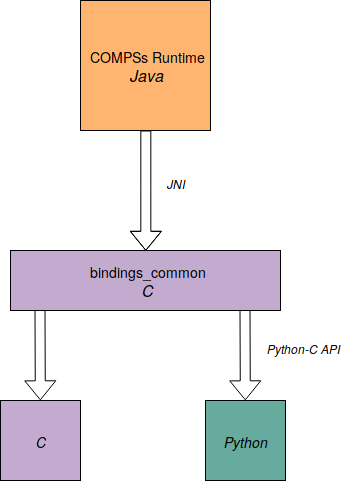
\includegraphics[scale=0.6]{estructuraBindings.png}
    \label{fig:estructura_bindings}
\end{figure}

\subsection{Modelo de ejecución en el binding C/C++}
\label{sec:bindings}

\textit{C} y \textit{C++} son lenguajes de programación compilados, esto quiere decir que necesitamos un segundo programa llamado compilador que procese nuestro programa y genere un fichero que nuestro ordenador pueda ejecutar, a este proceso se le llama compilar y al fichero generado, binario. De esta manera, para poder obtener el modelo de ejecución introducido en la sección \ref{modeloejecucion}, necesitaremos compilar dos binarios, uno para el \textit{master} y otro para los \textit{workers}.
\par\bigskip

\begin{comment}
La aplicación que desarrolla el usuario, \textit{a priori} no envía las tareas a ejecutar ni las dependencias entre estas, no gestiona el \textit{runtime}, pero es desarrollada siguiendo unas directrices que nos permitirán generar código que sí gestione todo lo que es necesario con tal de que la aplicación se distribuya correctamente. 
\end{comment}

La aplicación que desarrolle el usuario, tiene que ser transparente al \textit{runtime}, para conseguirlo tan sólo se necesita una interfaz indicando las tareas a detectar al ejecutar la aplicación. Entonces, una vez compilemos la aplicación de COMPSs en C/C++, se generará automáticamente (a partir de ahora \textit{autogenerar}) código para las tareas, que gestionarán la comunicación con el \textit{runtime}.
\smallskip
La siguiente imagen describe de manera visual cómo se compila una aplicación. 

\begin{figure}[H]
    \centering 
    \caption{Proceso de compilación de una aplicación COMPSs C/C++.}
    %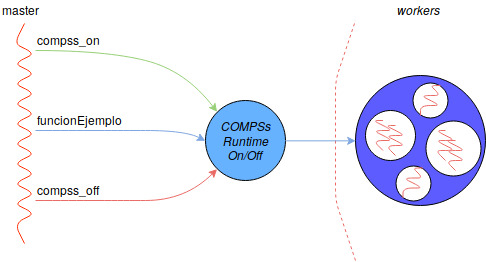
\includegraphics[width=\textwidth]{sta-masterworker.jpg}
    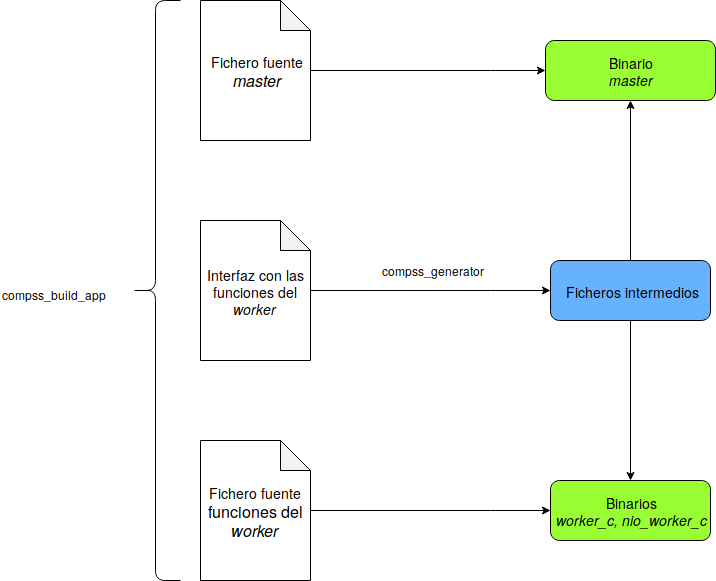
\includegraphics[scale=0.5]{workflowCompilado.png}
    \label{fig:workflowcompilado}
\end{figure}

\par\bigskip
Para facilitar el compilado de la aplicación se utiliza el script \textit{compss\_build\_app}, y para hacer la generación de código a partir de la interfaz, el binario \textit{compss\_generator}.
La aplicación una vez desarrollada por el usuario, compilada sin \textit{COMPSs} por el medio también funcionaría, pero sencillamente las tareas serían ejecutadas \textit{in situ} en el \textit{master}.  Lo que pretendemos hacer al introducir \textit{COMPSs} es que el \textit{master}, en vez de ejecutar la tarea, comunique al \textit{runtime} que se debe ejecutar una tarea, y este se encargue de ejecutarla en un \textit{worker}, todo evidentemente, de manera transparente al usuario.
\par\bigskip

\bigskip
En la figura \ref{fig:workflowcompilado} veíamos la caja negra de ficheros intermedios, estos ficheros son el \textit{stubs} y \textit{executor} (siempre del estilo, \textit{ejemplo-stubs.cc} y \textit{ejemplo-executor.cc} donde ejemplo es el nombre de la aplicación compilada). El fichero \textit{stubs} corresponde con la parte del \textit{master} que se encargará de comunicarse con el \textit{runtime} para registrar la tarea. Esto lo consigue implementando las funciones de las tareas con el código para gestionar su registro, es decir, sustituyendo el código que sería propio de la ejecución de cada tarea por un código para efectuar el registro en el \textit{runtime}. Una vez registrada la tarea, eventualmente el \textit{runtime} designará a un \textit{worker} a ejecutarla. El \textit{worker} recibirá la tarea que debe ejecutar, los datos necesarios y más parámetros, el \textit{executor} ha sido \textit{autogenerado} con el código principal de la aplicación, por lo que conoce como gestionar los datos y parámetros recibidos para ejecutar la tarea pertinente. 

\begin{comment}
\begin{figure}[H]
    \centering  
    \caption{Registro y ejecución de tareas en una aplicación COMPSs C/C++.}
    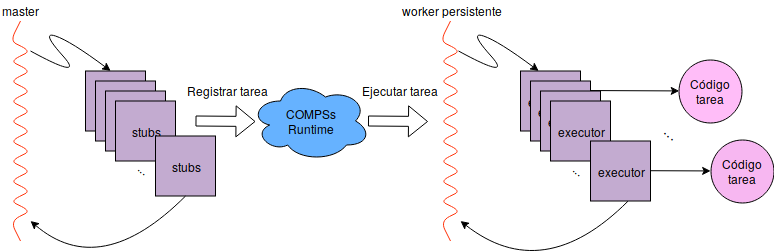
\includegraphics[scale=0.6]{stubs-executor.png}
    \label{fig:stubs-executor}
\end{figure}

La imagen anterior muestra las llamadas a funciones pertinentes a \textit{stubs} que contienen el código para registrar las tareas en el \textit{runtime}, la eventual ejecución de las tareas registradas en los \textit{workers} que haya disponibles y como toma parte su ejecución mediante el \textit{executor}. Ahora que sabemos como se estructura un \textit{binding}, y en concreto, como funciona el de \textit{C/C++}, el siguiente paso es estudiar el funcionamiento de \textit{OmpSs-2}.

%\subsection{Conceptos básicos de OmpSs-2}

\subsubsection{Mercurium}

\textit{Mercurium} es el encargado de compilar una aplicación de \textit{OmpSs-2} y hacer que las directivas insertadas en el código tengan efecto sobre este. De manera superficial, lo que hace es añadir código para gestionar el \textit{runtime}, encender el \textit{runtime}, añadir las tareas, notificar las dependencias y un largo etcétera. 

\subsubsection{Nanos6}

\todo{Pensar algo}
\end{comment}

\subsection{Modo librería: nanos6\_spawn\_function \label{spawnfunction}}

En la sección \ref{sec:bindings} dimos una visión más interna y propia de desarrollador del \textit{binding} de \textit{C/C++}. Sobre \textit{OmpSs-2} necesitamos saber, como se desarrolla una aplicación, en concreto con el modo librería.
\medskip

Esta funcionalidad, nos permite registrar una tarea en el \textit{runtime} de \textit{OmpSs-2} de manera asíncrona, con lo cuál podremos brindar a cada tarea y sus sucesoras un entorno aislado del resto. Gracias a esto, conseguiremos arreglar el problema con la migración de \texit{threads}, planteado en la sección \ref{compssompss}. \smallskip

\begin{lstlisting}[caption={Definición de la función nanos6\_spawn\_function.},captionpos=b, label={lst:nanos6spawn}, language=C++]
void nanos6_spawn_function(
   void (*function)(void *), 
   void *args,
   void (*completion_callback)(void *), 
   void *completion_args, 
   char const *label
);
\end{lstlisting}

La anterior imagen muestra la definición de la función que nos permitirá registrar una función \textbf{function} con argumentos \textbf{args} en el \textit{runtime}. Una vez ejecutada la función registrada como tarea, se ejecutará la función \textbf{completion\_callback} con argumentos \textbf{completion\_args} (mecanismo conocido como \textit{callback}, de ahí el nombre), el argumento de la función \textit{label} sirve para etiquetar la tarea con el nombre que contenga.

\subsubsection{Ejemplo}

Con tal de entender como funciona un programa que utilice el modo librería, vamos a ver un ejemplo sencillo. Este programa de ejemplo, hará \textit{spawn} de una función y dentro de ésta se generarán tareas con dependencias entre ellas. \smallskip

\begin{lstlisting} [caption={Función a ser registrada como tarea.},captionpos=b, label={lst:nanos6\_ejemplo}, language=C++]
 int nanos6_ejemplo(int* a) {

    int local_a;

    #pragma oss task shared(local_a) out(local_a) 
    {
        local_a = a[0];
    }

    #pragma oss task shared(local_a) inout(local_a)
    {
        local_a = local_a * 4;
    }

    #pragma oss taskwait

    return local_a;
}
\end{lstlisting}

En la imagen podemos ver la función \textbf{nanos6\_ejemplo}, ésta tiene como parámetro un puntero a enteros \textbf{a} y retorna un valor del tipo \textbf{int}. La función será registrada como tarea desde otro fichero. El cálculo que se realiza en la función no tiene la menor importancia, es solo un \textbf{ejemplo}. \medskip

Por supuesto, esta función será compilada con \textit{Mercurium}, si no fuera el caso, la función se ejecutaría correctamente pero no se generarían las tareas de dentro de la función, por lo cuál la ejecución sería secuencial. 

\begin{lstlisting} [caption={Gestión del modo librería desde el main.},captionpos=b, label={lst:library-main}, language=C++]
    char const *error = nanos6_library_mode_init();
    if (error != NULL)
    {
        fprintf(stderr, "Error initializing Nanos6: %s\n", error);
        return 1;
    }

    condition_variable_t cond_var = COND_VAR_INIT;

    ejemplo_wrapper_args_t args;

    int A = 1;
    args.array = &A;
    
    nanos6_spawn_function(ejemplo_wrapper, &args, 
    condition_variable_callback, &cond_var, 
    "spawned ejemplo");

    wait_condition_variable(&cond_var);

    printf("%li\n", args.ret);

    nanos6_shutdown();

\end{lstlisting}

Las funciones \textit{nanos6\_library\_mode\_init()} y \textit{nanos6\_shutdown()} efectúan respectivamente el encendido y apagado del \textit{runtime}, el código que vemos entre estas dos llamadas es el correspondiente para registrar una función como tarea utilizando el modo librería. Dado que la función nanos6\_spawn\_function espera como un puntero los parámetros a pasar a la función, se deben incluir todos dentro de una estructura que los pueda contener, el \textit{struct} \textit{ejemplo\_wrapper\_args\_t} tiene los campos \textbf{a} y \textbf{ret} que corresponden al parámetro de la función \textit{nanos6\_ejemplo} y valor de retorno de ésta.

\bigskip
Un detalle que no se ha comentado es que la ejecución de este código será efectuada por \textit{pthreads}, el estándar \textit{POSIX} de \textit{threads}. Dado que la ejecución de la tarea tendrá lugar de manera \textbf{asíncrona} es necesario un mecanismo de sincronización, la implementación de \textit{threads} que utilizamos (y por tanto los mecanismos de sincronización dependerán de estos) es la explicada en el apéndice \ref{appendix:pthread}.

\bigskip

Como es necesario utilizar una estructura auxiliar para pasar los parámetros mediante un puntero, necesitaremos también una función intermedia con la cuál llamar a la función que realmente queremos registrar como tarea. Habitualmente a este tipo de funciones intermedias se les llama \textit{wrapper}. En la siguiente imagen veremos la función que actúa como \textit{wrapper} de la función \textit{nanos6\_ejemplo}. \smallskip

\begin{lstlisting} [caption={Wrapper de la función nanos6\_ejemplo.},captionpos=b, label={lst:library-wrapper}, language=C++]
 void ejemplo_wrapper(void *untyped_arg)
{
    ejemplo_wrapper_args_t *args = 
        (ejemplo_wrapper_args_t *) untyped_arg;
    args->ret = nanos6_ejemplo(args->a);
}
\end{lstlisting}

El puntero de tipo \textit{void} puede contener cualquier tipo de estructura, aprovechando que sabemos que únicamente deberá contener el tipo \textit{ejemplo\_wrapper\_args\_t} se hace un \textit{cast} para interpretarlo como la estructura deseada. Se asigna \textbf{ret} al valor de retorno y se pasa \textbf{a} como parámetro.

\todo{faltan detalles de compilado...}

\subsection{Integración}

Ahora que tenemos claro el funcionamiento de ambas partes, podemos plantear un prototipo de la integración e implementarlo. Está claro que \textit{OmpSs-2} tomará parte únicamente en los nodos del tipo \textit{worker}, ya que es dónde realmente se ejecutarán las tareas detectadas por el \textit{master}. 
\par\medskip

En el ejemplo para utilizar el modo librería \ref{spawnfunction}, aprendimos como activar el \textit{runtime} de \textit{OmpSs-2} en este modo y como ejecutar las tareas, por lo que bastará con activarlo en los \textit{workers} (persistente y no persistente) y modificar la generación del código \textit{executor} (queremos hacerlo en el \textit{worker}) para generar la misma estructura del ejemplo en cada tarea de la interfaz de la aplicación.
\par\medskip
Entonces, con la activación de \textit{OmpSs-2} en los nodos \textit{worker} conseguiremos la siguiente estructura y modelo de ejecución.

\begin{figure}[H]
    \centering 
    \caption{Estructura y modelo de ejecución master-worker de la integración COMPSs+OmpSs-2}
    %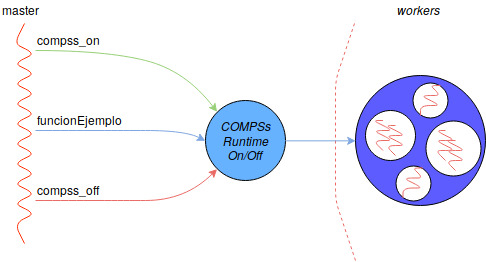
\includegraphics[width=\textwidth]{sta-masterworker.jpg}
    \includegraphics[scale=0.5]{compss2rt.png}
    \label{fig:compssompssrt}
\end{figure}

Durante la ejecución del programa principal se irá generando un grafo con las tareas que se deben ejecutar, eventualmente cada una de estas será enviada a un nodo \textit{worker} (en la figura tan sólo aparece uno, pero podrían ser más) y este ejecutará la tarea de \textit{COMPSs} en forma de tarea de \textit{OmpSs-2}.
La ejecución de las tareas de \textit{OmpSs-2} generará otro grafo, dónde figurarán tanto las tareas que han sido creadas mediante el mecanismo de \textit{spawn} como las que puedan ser creadas dentro de las anteriores, y finalmente las tareas de este grafo serán ejecutadas.

\subsubsection{Encendido y apagado del modo librería}

\todo{nio worker c y worker c}

\subsubsection{Generación del código de cada tarea}

\todo{spawn en sí}

\subsubsection{Modificaciones en la compilación actual}

\todo{modificacion de los scripts, autotools, etc}

\subsubsection{Tipo enum y cabeceras en la interfaz}

\todo{Añadido del tipo enum y el include de las cabeceras}

\section{Aplicación COMPSs+OmpSs-2}



\section{Estudio del rendimiento}

































\chapter{Evaluación}
\label{sec:estudiorend}

En este capítulo describiremos las aplicaciones descritas para evaluar la integración \textit{COMPSs+OmpSs-2}, los entornos donde haremos la evaluación y los resultados de esta.  

\section{Aplicaciones}
\subsection{K-Means}

\textit{K-Means} es un algoritmo utilizado para hacer \textit{clustering} sobre un grupo de datos, es decir, agrupar los datos en \textit{clusters}. Cada dato pertenece al \textit{cluster} cuyo centro está en la distancia mínima, si no fuera así pertenecería a otro \textit{cluster}. Se inicializan \textit{clusters} con centros escogidos de manera aleatoria y se comparan las distancias a todos los \textit{clusters} y se determina a cual pertenece cada dato (siempre al centro más cercano), una vez hecho esto se vuelve a calcular el centro de cada \textit{cluster}, todo este proceso conforma una iteración de \textit{K-Means}, habitualmente se itera hasta que converge, esto es que la distancia entre los centros asignados en dos interaciones consecutivas de cada \textit{cluster} es cercana a 0.

\begin{figure}[h]
	\centering 
	\caption{Grafo de dependencias entre tareas de K-Means.}
	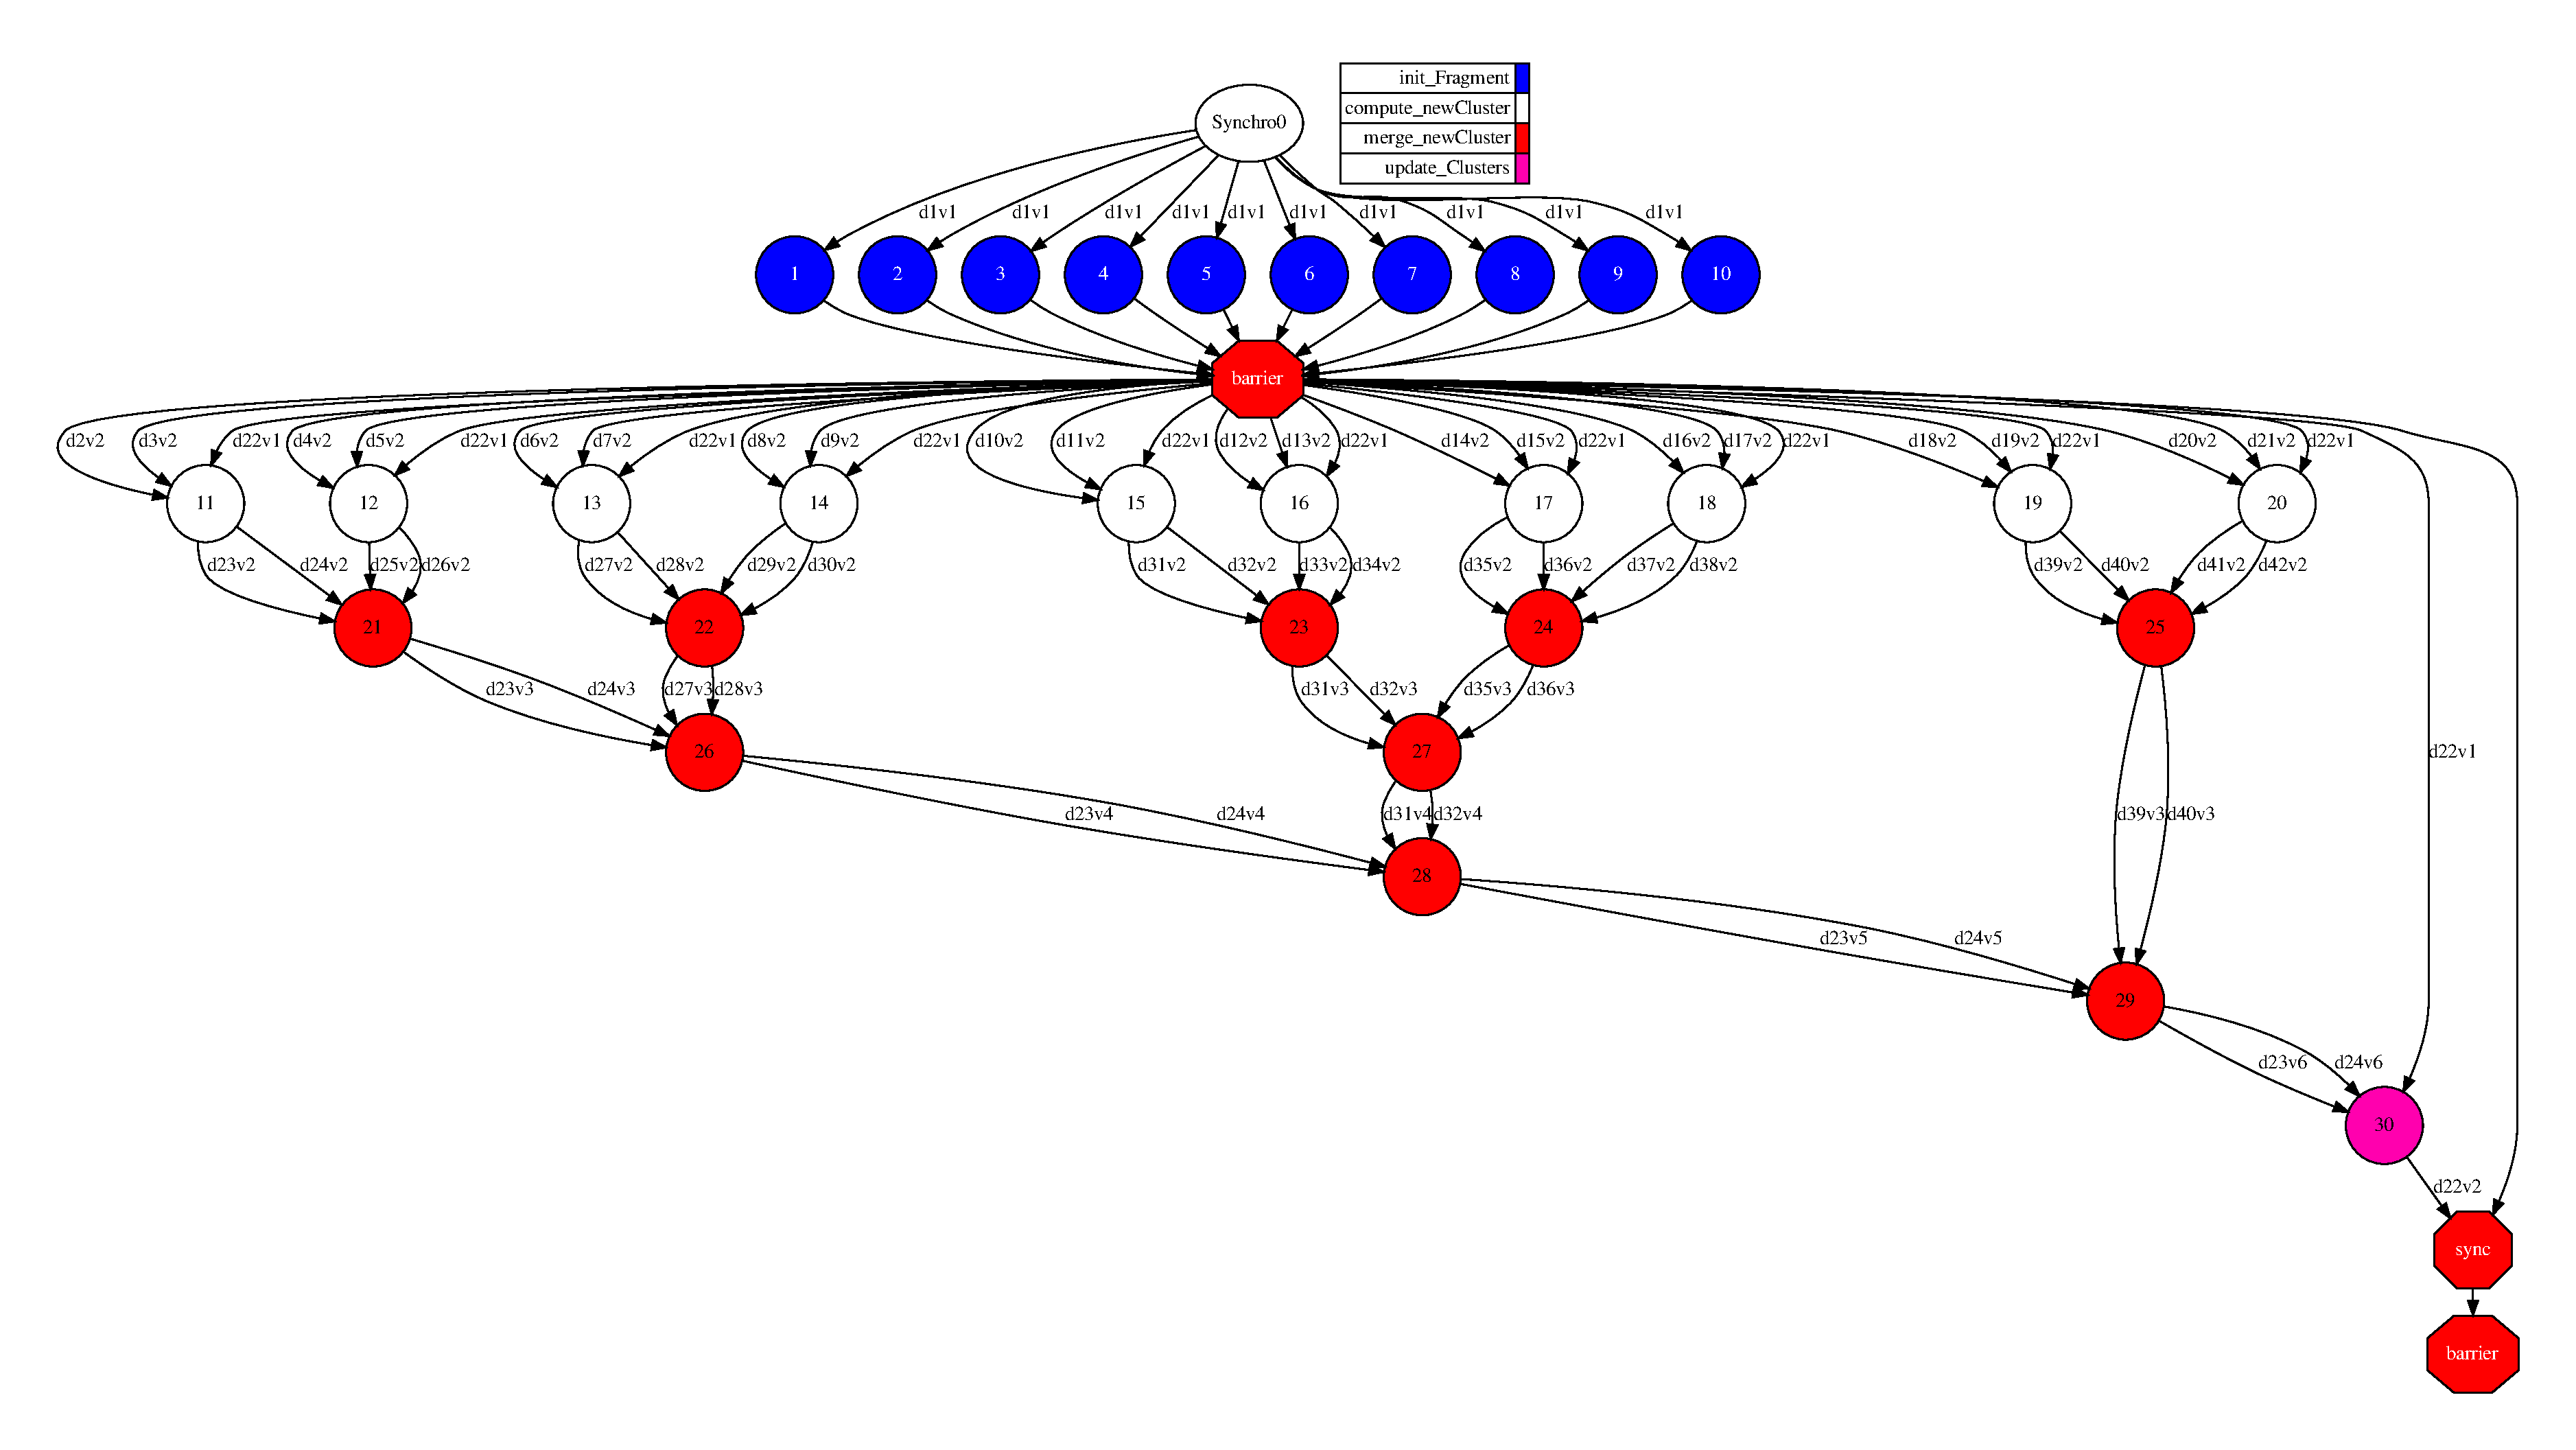
\includegraphics[scale=0.2]{grafo_kmeans.pdf}
	\label{fig:grafokmeans}
\end{figure}

Tal y como hemos desarrollado la aplicación tiene 4 tareas, que son \textit{init\_Fragment}, \textit{compute\_newCluster} (tiene una implementación en CPU y otra en GPU), \textit{merge\_newCluster}, \textit{update\_Clusters}. La imagen \ref{fig:grafokmeans} muestra un grafo de dependencias de una ejecución de \textit{K-Means} donde el número de \textit{clusters} a formar es 25 y se efectúa una única iteración. Para no sobrecargar este apartado se incluye en el apéndice \ref{sec:codigokmeans} la interfaz y el programa principal de la aplicación.

\subsection{Cholesky}

\textit{Cholesky} es un método de descomposición aplicable cuando la matriz es simétrica definida positiva, entonces esta puede ser descompuesta como el producto de una matriz triangular inferior y su traspuesta. El método \textit{Cholesky} se utiliza para resolver sistemas de ecuaciones lineales, es similar a la descomposición \textit{LU} y es el doble de eficiente.
\par\bigskip
La aplicación ha sido desarrollada utilizando una librería para operaciones de algebra lineal programada en \textit{C} con \textit{OmpSs} y \textit{OmpSs-2}, esta librería es \textit{LASs}\footnote{https://pm.bsc.es/mathlibs/lass} (\textit{Linear Algebra routines on OmpSs}). Las funciones que implementa \textit{LASs} serán utilizadas como tareas a nivel de \textit{COMPSs} y después una vez ejecutadas harán uso de \textit{OmpSs-2}, por lo que realmente desarrollar una aplicación utilizando una librería externa es muy sencillo.
\par\bigskip
Tiene 5 tareas, \textit{generate\_block}, \textit{ddss\_dpotrf}, \textit{ddss\_dtrsm}, \textit{ddss\_dgemm}, \textit{ddss\_dsyrk}, \textit{generate\_block} se utiliza para generar los bloques de manera distribuida (así el \textit{master} no tiene reservar memoria para toda la matriz, que podría ser muy grande), las otras 4 tareas son operaciones de algebra lineal que utilizadas de la forma correcta aplicarán el método de descomposición de \textit{Cholesky}.
En el apéndice \ref{sec:codigocholesky} se encuentra la interfaz y el programa principal de la aplicación. 

\begin{figure}[h]
	\centering 
	\caption{Grafo de dependencias entre tareas de Cholesky.}
	\includegraphics[scale=0.07]{grafo_cholesky.pdf}
	\label{fig:grafocholesky}
\end{figure}

La imagen \ref{fig:grafocholesky} muestra un grafo de dependencias de la aplicación \textit{Cholesky} con una matriz de 64 bloques con 4096x4096 elementos cada uno. 

\section{Entornos para el estudio}

Para la realización del estudio del rendimiento se han utilizado dos máquinas que el \textit{Barcelona Supercomputing Center} pone a nuestra disposición, que son \textit{CTE-Power} y \textit{MareNostrum4}.

\subsection{CTE-Power}
\label{sec:power}

\textit{CTE-Power} es un \textit{cluster} basado en la tecnología de procesadores \textit{IBM} \textit{Power9}. Tiene 2 nodos de \textit{login}, son los nodos desde donde operan los usuarios y 52 nodos de cómputo. 
\par\smallskip
Cada nodo tiene los siguientes componentes:
\par\smallskip
\begin{itemize}
	\item 2 x \textit{IBM Power9 8335-GTH} @ 2.4GHz (3.0GHz en modo turbo), cada procesador con 20 cores cada uno con 4 \textit{threads}.
	\item 512GB de memoria organizada en 16 \textit{dimms} de 32GB @ 2666MHz.
	\item 4 x \textit{NVIDIA} V100 con 16GB \textit{HBM2}.
	\item 2 x SSD que proporcionan 1.9TB de almacenaje local.
	\item 2 x \textit{NVM Express} 3.2TB.
	\item Interfaz de red \textit{Mellanox}.
	\item Sistema de ficheros GPFS a través de fibra a 10GBit.
\end{itemize}

Nosotros utilizaremos tan sólo 10 nodos, por lo que tendremos a nuestra disposición en la mayor ejecución 1600 CPUs y 40 GPUs \textit{NVIDIA V100}. 

\subsection{MareNostrum4}
\label{sec:mare}

\textit{MareNostrum4} es un supercomputador basado en la tecnología de procesadores \textit{Intel Xeon Platinum} de la generación \textit{Skylake}. Tiene 5 nodos de \textit{login} y 3.456 nodos de cómputo.
\par\smallskip
Cada nodo tiene los siguientes componentes:
\par\smallskip
\begin{itemize}
	\item 2 x \textit{Intel Xeon Platinum 8160 @ 2.10GHz} con 24 cores.
	\item Hay nodos con distintos tipos de memoria:
		\subitem 1,88 GB/core de memoria. %organizada en 12 \textit{dimms} de 8GB @ 2667MHz.
		\subitem 7,93 GB/Core de memoria.
	\item Un SSD que proporciona 200 GB de almacenaje local.
	\item 100 Gbit/s \textit{Intel Omni-Path HFI Silicon 100 Series PCI-E adapter}.
	\item 10 Gbit \textit{Ethernet}.
\end{itemize}

Igual que con \textit{CTE-Power} tan sólo utilizaremos 10  nodos, por lo tanto tendremos en la mayor ejecución 480 CPUs.

\section{K-Means}

La evaluación con \textit{K-Means} ha consistido en hacer un test de \textit{strong scaling}, que consiste en ejecutar la aplicación con un tamaño de problema fijo y aumentar el número de recursos de cómputo, y otro de \textit{weak scaling} donde aumentaremos de manera proporcional el tamaño del problema y los recursos de cómputo. En el apartado \ref{sec:power} describimos la máquina que utilizamos en estos test, haremos uso de todas las \textit{CPUs} y \textit{GPUs} de cada nodo.

\subsection{Strong scaling}

La imagen \ref{fig:sc-time} muestra una gráfica que tiene en el eje vertical el tiempo y en el horizontal el número de nodos. El tamaño del problema que se ha utilizado es de 400 fragmentos de 50 dimensiones y 200000 puntos cada uno, el número de \textit{clusters} a formar es 50 y se efectúan 5 iteraciones. Se han tomado 10 muestras de cada ejecución, la línea azul muestra la media de las muestras para el mismo número de nodos, la de color naranja muestra el tiempo ideal que debería tardar según el número de nodos. En cada punto de la línea azul se muestra la diferencia entre el máximo valor y el mínimo que se han tomado en las muestras.

\begin{figure}[H]
	\centering 
	\caption{Tiempo de ejecución al aumentar el número de recursos.}
	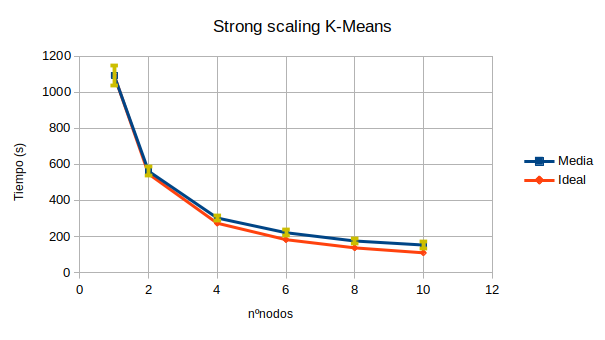
\includegraphics[scale=0.8]{estudio/KMeans/sc/kmeans-sc-time.png}
	\label{fig:sc-time}
\end{figure}

Es bueno que la línea azul sea lo más parecida a la línea naranja, eso nos indicaría que la aplicación escala perfectamente, ya que cada vez que aumentamos los recursos el tiempo de ejecución se reduciría proporcionalmente. La imagen \ref{fig:sc-speedup} muestra la misma información que \ref{fig:sc-time} dispuesta en forma de ganancia, se puede ver que se comporta bien hasta que en los 6 nodos empieza a dejar de acercarse al ideal.

\begin{figure}[H]
	\centering 
	\caption{Ganancia al aumentar el número de recursos.}
	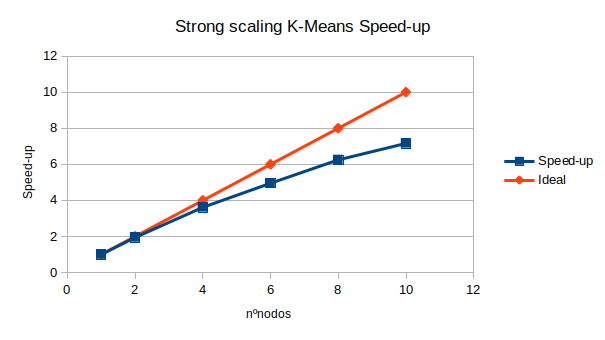
\includegraphics[scale=0.8]{estudio/KMeans/sc/kmeans-sc-speedup.png}
	\label{fig:sc-speedup}
\end{figure}

\subsection{Weak scaling}

En un test de \textit{weak scaling}, esperamos que los tiempos de ejecución sean siempre los mismos, ya que el tamaño del problema es siempre proporcional a los recursos de cómputo. Esto sería perfecto pero hay que efectuar comunicación entre nodos y gestionar todo el sistema, por lo que no podemos mantener este escenario ideal. La imagen \ref{fig:wc-effic} muestra cómo al aumentar el número de nodos la eficiencia baja del ideal (que el tiempo de ejecución sea siempre el mismo), pero se mantiene alrededor del mismo valor a partir de los 6 nodos.

\begin{figure}[H]
	\centering 
	\caption{Eficiencia al mantener proporcional el tamaño del problema y el número de recursos.}
	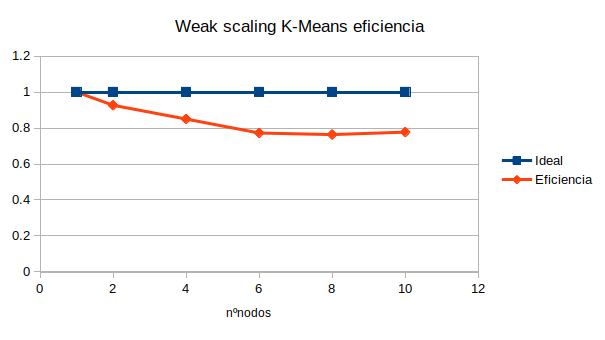
\includegraphics[scale=0.8]{estudio/KMeans/wc/kmeans-wc-efficiency.png}
	\label{fig:wc-effic}
\end{figure}

\section{Cholesky}











\newpage

\appendixpage
\appendix
\section{Planificación temporal}
\label{sec:planificacion}

Esta sección presenta como se utilizarán los aproximadamente cuatro meses de duración que tiene el proyecto, desde Febrero de 2019 hasta Junio de 2019. Se especificarán las tareas a realizar junto a su durada aproximada, teniendo en cuenta las posibles desviaciones en la realización de estas. Dado que cualquier desviación puede resultar en la alteración de la planificación, se debe tener en cuenta que la especificación que sigue no debe tomarse al pie de la letra, sino que debe reinterpretarse y modificarse siempre que sea necesario. 

\subsection{Especificación de las tareas}

Detallamos a continuación las tareas a realizar.

\subsubsection{GEP - Gestión de proyectos}

La asignatura GEP conforma el primer bloque del proyecto, se debe elaborar cuatro entregables que sinteticen la temática del proyecto, objetivos, como se realizará (metodología), definir las actividades, realizar un estudio de sostenibilidad y finalmente presentar este documento con soporte visual de manera oral ante un tribunal.

\begin{itemize}
 \item \textbf{Elaboración del primer entregable:} En este primer apartado se dará un contexto, el estado del arte del proyecto, los objetivos, requerimentos, riesgos y una metodología para desarrollar el proyecto en sí. La duración aproximada es de unas 24 horas.
 \item \textbf{Elaboración del segundo entregable:} En este apartado se definen las actividades y duración de estas. La duración aproximada es de 6 horas.
 \item \textbf{Elaboración del tercer entregable:} En este apartado se realizará la autoevaluación sobre la sostenibilidad además de un análisis sobre la gestión económica y la sostenibilidad del proyecto. La duración aproximada es de 18 horas.
 \item \textbf{Elaboración del cuarto entregable:} En este último apartado se preparará una presentación oral y se confeccionará el documento final, que serán los tres anteriores revisados y corregidos con la orientación del \textit{feedback} del profesor de GEP, director y codirector. La duración aproximada es de 12 horas.
\end{itemize}

Con estos cuatro apartados se finaliza el GEP. En princpio, la duración estipulada del GEP es de 75 horas, la suma de las horas que hemos creído que durarían es de 60 horas, esta diferencia nos proporcionará cierto margen para corregir y mejorar los entregables. Para realizar esta actividad, se empleará un ordenador, \textit{GitHub} para subir la documentación, \textit{Kile} para redactar el documento en \textit{LaTeX},\textit{Trello} para organizar las actividades en forma de tarjetas, \textit{Gantter} para elaborar el diagrama de \textit{Gantt} y \textit{Google Drive}.

\subsubsection{Uso de la API de Nanos6}

Para poder llevar acabo exitosamente la integración, se necesita entender qué hace y saber utilizar la \textit{API} de \textit{Nanos6}. Requiere mirar documentación e interactuar con los desarrolladores de \textit{Nanos6}. 
\par\bigskip

Queremos aprender a utilizar la llamada \textit{nanos6\_spawn\_function}, que nos permitirá ejecutar una función como tarea. Para poder utilizarla, necesitamos levantar el \textit{runtime} de manera manual en un programa compilado con \textit{gcc} (\textit{GNU C Compiler}) o bien \textit{g++} cuando se utilice \textit{C++}, y efectuar la llamada a una función externa compilada con \textit{mcc} (\textit{Mercurium}), ya que estará anotada con pragmas de \textit{OmpSs-2}.
\par\bigskip

El tiempo aproximado para realizar esta tarea es de 60 horas. Los recursos necesarios son un ordenador con un compilador nativo de \textit{C}, otro de \textit{C++}, y \textit{Mercurium} y \textit{Nanos6} instalados. 

\subsubsection{Integrar OmpSs-2 en el binding de C/C++}

La tarea principal que da sentido al proyecto es esta, comprende el estudio y la integración de \textit{OmpSs-2} en el \textit{binding} de \textit{C/C++}. Requiere del estudio de la estructura interna de \textit{COMPSs} por una banda y del \textit{binding} por otra, con tal de saber dónde se podría inicializar el \textit{runtime} de \textit{Nanos6} y cuándo se debería apagar. También se necesita hacer la llamada a la \textit{API} en el \textit{worker}, cosa que habrá que estudiar también dónde situar.
\par\bigskip

El primer paso consistirá en analizar dónde tendría más sentido que hagamos la gestión del \textit{runtime} de \textit{Nanos6}, y cómo hacerla. Para esto tendremos que dar un repaso al código de \textit{COMPSs} y determinar qué hace cada componente de este. 
%\par\bigksip

En segundo lugar se deberá implementar toda la gestión. Se deberá también estudiar dónde se debería hacer la llamada a la \textit{API}, y por verificar el funcionamiento de la integración, que será de seguro lo más complejo y lo que más tiempo requerirá.
%\par\bigskip

Esta tarea es la que más tiempo nos llevará, ya que será el primer intento serio de integrarlo todo, pero nos aportará conocimiento pleno de como funciona y por lo tanto facilidad para trabajar en futuras ampliaciones. La duración será aproximadamente de 96 horas. Los recursos necesarios son un ordenador con \textit{COMPSs} instalado, un compilador nativo de \textit{C}, otro de \textit{C++}, y \textit{Mercurium} y \textit{Nanos6} instalados.

\subsubsection{Estudiar la integración de OmpSs-2 en Java y binding de Python}

En caso de que la primera integración haya funcionado, se estudiará la posibilidad de hacer lo mismo con \textit{Java} y el \textit{binding} de \textit{Python}. Consistirá exactamente de los mismos pasos, y puede ayudar a mejorar la implementación anterior. La duración estimada de esta tarea dependerá de si se decide realizar o no esta actividad. Mínimo se emplearán 15 horas en el estudio preliminar, y en caso de realizar la integración, 78 horas más, es decir, 15 horas o bien 93 horas. Pese a que la tarea es muy similar a la anterior, el tiempo previsto es algo menor por el hecho de que ya se ha podido realizar una integración y la implementación debería ser parecida. Los recursos necesarios son un ordenador con \textit{COMPSs} instalado, un compilador nativo de \textit{C}, otro de \textit{C++}, y \textit{Mercurium} y \textit{Nanos6} instalados.

\subsubsection{Estudio previo del rendimiento}

Dado que este proyecto parte de la premisa de resolver unos problemas concretos con el rendimiento, se efectúa un estudio muy concreto hacia estos problemas para ver si están resueltos o no. Que este estudio vaya mal o no, no afecta realmente al proyecto, ya que se intentará ver si \textit{OmpSs-2} mejora respecto a \textit{OmpSs} de todas formas.

\subsubsection{Desarrollo de una aplicación que use COMPSs+OmpSs-2}

En esta tarea se quiere desarrollar una aplicación que haga uso de \textit{COMPSs+OmpSs-2} con tal de estudiar después el rendimiento de la integración. La aplicación no puede ser cualquiera, ya que no toda aplicación mejorará su rendimiento conforme añadamos recursos heterogéneos. Dado que aún hay mucho margen, se ideará más adelante cuál será la aplicación a desarrollar. El tiempo que se empleará en esta tarea es de aproximadamente 84 horas. Los recursos necesarios son un ordenador con \textit{COMPSs} instalado, un compilador nativo de \textit{C}, otro de \textit{C++}, y \textit{Mercurium} y \textit{Nanos6} instalados.

\subsubsection{Estudio del rendimiento}

Utilizando la aplicación desarrollada en la tarea anterior estudiaremos el rendimiento de la integración, haremos uso de herramientas del \textit{BSC} como por ejemplo \textit{Extrae} y \textit{Paraver}, desarrolladas por el grupo \textit{Performance Tools} que nos permitirán extraer trazas para las tareas que ejecuten los \textit{workers} una vez la aplicación haya acabado y después visualizarlas. También haremos uso de opciones de \textit{COMPSs} para medir cuánto tarda cada tarea enviada a un nodo.
\par\bigskip

Estudiar el rendimiento incluirá intentar optimizar al máximo todas las pérdidas de rendimiento en la medida de lo posible, por lo cual el tiempo aproximado para llevarla a cabo, es de 84 horas. Los recursos necesarios son un ordenador con las herramientas mencionadas anteriormente instaladas, \textit{COMPSs} instalado, un compilador nativo de \textit{C}, otro de \textit{C++}, y \textit{Mercurium} y \textit{Nanos6} instalados.

\subsubsection{Redactar la memoria}

Por último se deberá redactar la memoria del proyecto además de preparar todo el material audiovisual para la defensa de este. La duración de esta actividad será de unas 72 horas. Los recursos que se utilizarán son \textit{Kile} para redactar el documento en \textit{LaTeX}, \textit{GitHub} para guardar la documentación y \textit{LibreOffice} para el apoyo audiovisual que se utilizará durante la defensa.

\subsection{Dependencias}

La siguiente tabla define la relación de dependencia entre las tareas que conciernen a la gestión del proyecto.

\begin{table}[H]
\centering
 \begin{tabular}{|| l | l ||}
    \hline  
    Tarea dependiente & Tarea predecesora \\
    \hline\hline
    Contexto & - \\
    \hline
    Estado del arte & Contexto \\
    \hline
    Objetivos, requerimentos, riesgos & Estado del arte \\
    \hline
    Metodología & Objetivos, requerimentos, riesgos \\
    \hline
    Definir actividades & Metodología \\
    \hline
    Estimar tiempos & Definir actividades \\
    \hline
    Autoevaluación sobre la sostenibilidad & Estimar tiempos \\
    \hline
    Análisis del proyecto & Autoevaluación sobre la sostenibilidad \\
    \hline
    Confeccionar documento final & Análisis del proyecto \\
    \hline
    Preparar presentación & Confeccionar documento final \\
    \hline
 \end{tabular}
 \caption{Relación de dependencia para las tareas de la gestión del proyecto.}
 \label{table:1}
\end{table}

La tabla anterior muestra la relación de dependencia, se respetará esta relación ya que las tareas a elaborar se agrupan y tienen fecha de entrega por separado. 

\begin{table}[H]
 \centering
 \begin{tabular}{|| l | l ||}
    \hline  
    Tarea dependiente & Tarea predecesora \\
    \hline\hline
    Uso de la API Nanos6 & GEP \\
    \hline
    Integrar OmpSs-2 en C/C++ & Uso de la API \\
    \hline
    Integrar OmpSs-2 en Java & Integrar OmpSs-2 en C/C++ \\
    \hline
    Integrar OmpSs-2 en Python & Integrar OmpSs-2 en Java \\
    \hline
    Estudio previo del rendimiento & Integrar OmpSs-2 en Python \\
    \hline
    Desarrollo aplicación COMPSs+OmpSs-2 & Estudio previo del rendimiento \\
    \hline
    Estudio del rendimiento & Desarrollo aplicación COMPSs+OmpSs-2 \\
    \hline
    Redactar la memoria & Estudio del rendimiento \\
    \hline
 \end{tabular}
    \caption{Relación de dependencia para las tareas de implementación del proyecto.}
    \label{table:2}
\end{table}

Salvo por algún motivo que implique bloquear una tarea, no se deberán adelantar tareas dependientes a las predecesoras, entre estos posibles motivos se contemplan errores en la implementación que nos bloqueen y se puedan ir haciendo otras cosas y cambios generales en las tareas a realizar.

\subsection{Estimación temporal de las tareas y recursos necesarios}

En el momento en el que se han enumerado y explicado las tareas se ha comentado la duración temporal y los recursos necesarios para cada actividad. En las siguientes dos secciones se recopilan estos datos en forma de tabla.

\subsection{Estimación temporal de las tareas}

\begin{table}[H]
 \centering
 \begin{tabular}{|| l | l ||}
  \hline
  Tarea & Estimación temporal (horas) \\
  \hline\hline
   Gestión del proyecto & 60 \\%& GitHub, Kile, Trello, Gantter, Google Drive \\
   \hline
   Uso de la API Nanos6 & 60 \\%& Compilador de C y C++, Mercurium, Nanos6 \\
   \hline
   Integrar OmpSs-2 en C/C++ & 96 \\%& COMPSs, Compilador de C y C++, Mercurium, Nanos6 \\
   \hline
   Integrar OmpSs-2 en Java y Python & 93 \\%& COMPSs, Compilador de C y C++, Mercuirum, Nanos6 \\
   \hline
   Desarrollo aplicación COMPSs+OmpSs-2 & 84 \\%& COMPSs, Compilador de C y C++, Mercurium, Nanos6 \\
   \hline
   Estudio del rendimiento & 84 \\%& COMPSs, Compilador de C y C++, Mercurium, Nanos6 \\
   \hline
   Redactar la memoria & 72 \\%& GitHub, Kile, LibreOffice \\
  \hline
  Total & 549 \\
  \hline
 \end{tabular}
 \caption{Estimación temporal de las tareas.}
\end{table}

En los apéndices 

\subsection{Recursos necesarios para las tareas}

\begin{table}[H]
 \centering
 \begin{tabular}{| l | l |}
 \hline
 Tarea & Recursos necesarios \\
 \hline\hline  
 Gestión del proyecto & GitHub, Kile, Trello, Gantter, Google Drive \\
 \hline
 Uso de la API Nanos6 & Compilador de C y C++, Mercurium, Nanos6 \\
 \hline
 Integrar OmpSs-2 en C/C++ & COMPSs, Compilador de C y C++, Mercurium, Nanos6 \\
 \hline
 Integrar OmpSs-2 en Java y Python & COMPSs, Compilador de C y C++, Mercurium, Nanos6 \\
 \hline
 Estudio del rendimiento & COMPSs, Compilador de C y C++, Mercurium, Nanos6 \\
 \hline
 Redactar la memoria & GitHub, Kile, LibreOffice \\
 \hline
 \end{tabular}
 \caption{Recursos necesarios para las tareas.}
\end{table}

En la tabla anterior, se muestran los recursos estrictamente necesarios para realizar la tarea, sin embargo, se ofrece ahora una lista de los recursos \textit{hardware} y \textit{software} que se utilizarán para la realización del proyecto en general. Además hay que tener en cuenta todos los recursos humanos necesarios.

\subsubsection{Recursos hardware}

\begin{itemize}

 \item \textbf{Ordenador portátil:} Proporcionado por el \textit{BSC}, Dell Latitude 7480 Intel® Core™ i7-6650U Processor (Dual Core, 4M Cache, 2.2GHz,15W, vPro), 512GB SSD (\textit{Solid State Drive}), Intel® HD Graphics 540 y 16 GB de memoria \textit{RAM}.
 
 \item \textbf{Pantalla:} Es habitual la configuración de portátil con una pantalla para simular una torre, la pantalla externa es también Dell, el modelo Professional P2217H.
 
 \item \textbf{Periféricos:} Todos los periféricos, ratón y teclado en este caso.
 
 \item \textbf{Clústers:} Con tal de medir el rendimiento ejecutando la aplicación que se desarrollará haciendo uso de la integración, necesitaremos un clúster con una arquitectura heterogénea. En la lista de candidatos se encuentran \textit{MinoTauro} y \textit{CTE-Power}, ambos están dotados de nodos que contienen \textit{CPUs} y \textit{GPUs}, se aprofundizará más en sus caracterísitcas en el momento de medir el rendimiento.
 
 \item \textbf{Puesto de trabajo:} El equipo de \textit{WDC} se encuentra en el edificio \textit{K2M}, allí es donde el desarrollador tendrá un puesto de trabajo y podrá desarrollar la mayoría del proyecto.
 
\end{itemize}

\subsubsection{Recursos software}

\begin{itemize}
    \item \textbf{Ubuntu 18.04:} Con tal de desarrollar se necesita un sistema operativo, el portátil tendrá instalado \textit{Ubuntu 18.04}.

    \item \textbf{GitHub y GitLab:} Para efectuar un control de versiones sencillo y eficaz, se utilizará el \textit{GitHub} personal del desarrollador para gestionar la documentación y el \textit{GitLab} del grupo \textit{WDC} para gestionar el código.

    \item \textbf{Editores: } Para editar código en \textit{Java} se utilizará \textit{IntelliJ IDEA}, para \textit{Python} \textit{PyCharm}, ambos de \textit{JetBrains}, y para C y C++ se utilizará \textit{Vim}.

    \item \textbf{Terminal: } La gran parte del tiempo se pasará entre terminales haciendo implementaciones y probando su funcionamiento, para hacer uso de un terminal se utilizará el emulador de terminales \textit{Terminator}.

    \item \textbf{Planificación y organización: } Para hacer el diagrama de \textit{Gantt} se ha utilizado \textit{Gantter} como extensión para \textit{Google Drive}. Además para organizarse y emplear la metodología \textit{SCRUM} se utilizará \textit{Trello}.

    \item \textbf{Compiladores y gestores de proyectos: } Para compilar código en C y C++ se utilizará \textit{gcc} y \textit{g++} respectivamente, para todo código que use \textit{OmpSs-2} se utilizará \textit{Mercurium}. El proyecto de \textit{COMPSs} está gestionado con \textit{Maven}, de esta manera se pueden generar todos los ficheros de \textit{Java} de manera sencilla. 
    
    \item \textbf{Software del proyecto: } Para poder desarrollar el proyecto, se precisará de una instalación de \textit{COMPSs}, \textit{Nanos6} y \textit{Mercurium}. Además, para medir el rendimiento se precisará de \textit{Extrae} y \textit{Paraver}. Con fines de \textit{debugging} se utilizará \textit{gdb}.

    \item \textbf{Editores de texto: } Para escribir el \textit{LaTeX} se utilizará \textit{Kile}.
\end{itemize}

\subsubsection{Recursos humanos}

\begin{itemize}
 \item \textbf{Director y codirector: } Efectuarán el seguimiento del proyecto de manera rutinaria y ayudarán a que el desarrollador sea capaz de llevarlo a cabo. 
 \item \textbf{Soporte: } Al utilizar \textit{software} de diversos proyectos, todas las personas que ayuden al desarrollador a solucionar problemas son recursos necesarios del proyecto.
 \item \textbf{Desarrollador: } Persona encargada de llevar a cabo en ultima instancia el proyecto.
\end{itemize}

\subsection{Valoración de alternativas y plan de acción}

En un proyecto de este tipo, es probable que haya desviaciones respecto el plan original. Esto es normal, tan sólo hay que saber cómo actuar ante estas desviaciones. Cualquier error en una implementación puede acarrear tiempo de más para solucionarlo, e incluso algo que se implementó hace mucho puede influir en las del futuro, por ello nuestra planificación intenta ser flexible, aún así, debemos planear como actuar en estos casos.

\begin{itemize}
 \item Si una tarea dura menos de lo esperado, sencillamente hay que coger la siguiente de la planificación y empezar a hacerla. Que una tarea dure menos que otra nos puede aportar un margen de acción muy útil.
 \item Si una tarea dura más tiempo de lo esperado, habrá que planteárselo de dos maneras, o bien se acorta otra tarea con tal de ajustarnos a la planificación o bien se intentan reducir lo mínimo posible los objetivos del proyecto para poderlo acabar en el tiempo establecido.
\end{itemize}

La tarea que más tiempo puede llevar dada la aparición de imprevistos es la de integrar \textit{OmpSs-2} en el \textit{binding} de C. Dado que la documentación aún está en una fase un tanto primeriza y no siempre tenemos por qué contar con el apoyo de soporte, por lo cuál habrá que invertir tiempo extra en ese caso. 
\par\medskip
El resto de tareas van un poco de la mano de esta anterior, no debería haber ninguna complicación extra. Como mucho en el estudio del rendimiento podemos encontrar resultados que no nos gusten o no acaben de agradar del todo, pero es parte del proyecto, se intentará mejorar dentro del tiempo estipulado. 
\par\medskip
Por tanto, siempre que falte tiempo para realizar una tarea se intentará equilibrar entre el resto, ya que el riesgo de sufrir un imprevisto es bastante bajo.
\par\bigskip
Para ser más previsores, en las reuniones de seguimiento se intentarán prever estos posibles problemas durante la realización del proyecto. 



















\newpage


\begin{landscape}
\appendixpage
\appendix
\section{Planificación y diagrama de Gantt correspondiente}

\begin{figure}[H]
    \centering 
    \caption{Tareas definidas para el diagrama de Gantt.}
    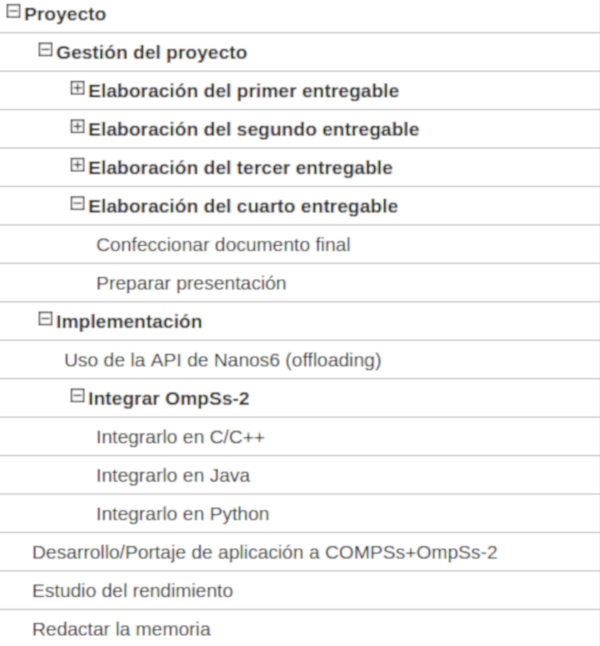
\includegraphics[scale=2.5]{ganttProyecto.png}
    \label{fig:gantt_tareas}
\end{figure}

\begin{figure}[H]
    \centering 
    \caption{Diagrama de Gantt del proyecto.}
    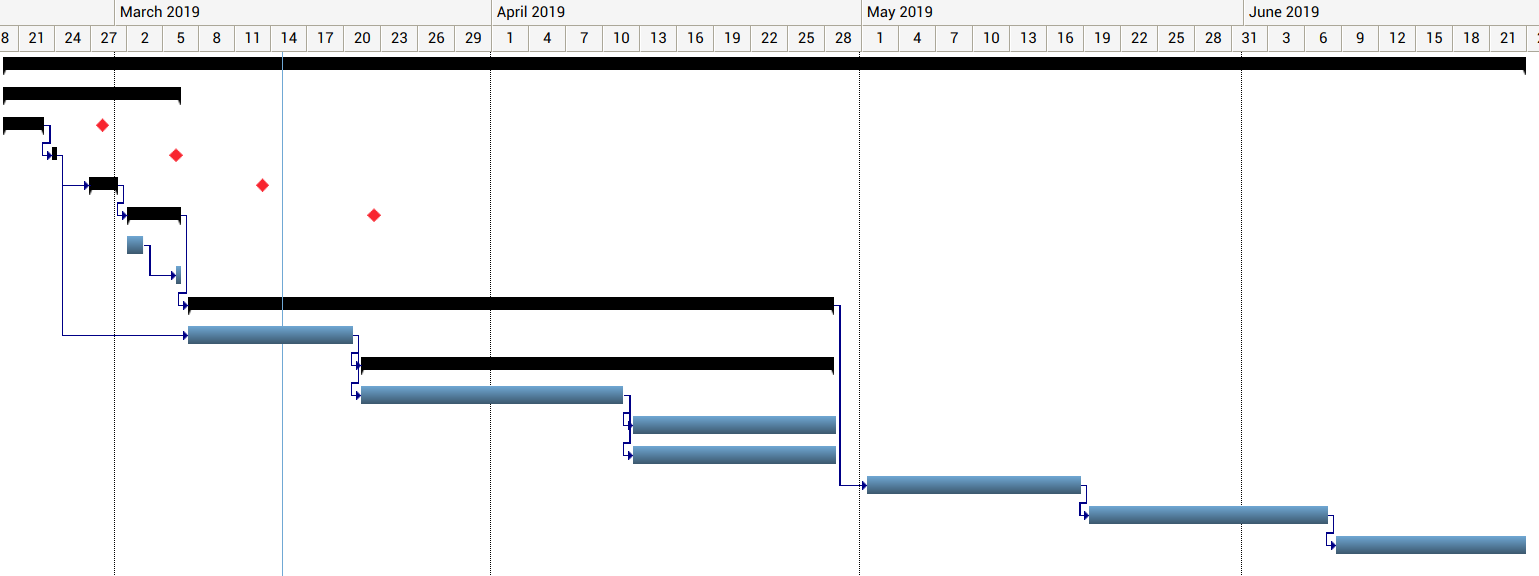
\includegraphics[scale=2]{diagramaGantt.png}
    \label{fig:diagrama_gantt}
\end{figure}
\end{landscape}

\newpage
\section{Autoevaluación sobre la sostenibilidad}

Todos los alumnos que estén realizando un trabajo de final de grado este cuatrimestre, saben qué supone el impacto de un proyecto sobre la sostenibilidad. Es difícil para mí, analizar de manera crítica y de alguna manera metódica estos impactos que se describen en la encuesta. 
\par\medskip
En cuanto a conocer los impactos, tener sentido común e intentar siempre reducir los impactos que de alguna manera sean insostenibles, sí que hay un conocimiento pleno y ganas de mantenerlo, pero desconozco los métodos más avanzados y profesionales para abordar la reducción de impactos negativos y aumentar la sostenibilidad de un proyecto.
\par\medskip
Los aspectos ambientales son de alguna manera los que resultan más intuitivos, de manera que no resulta difícil desenvolverse en primer momento, pero no conozco en profundidad el tema.
\par\medskip
En cuánto a aspectos sociales, de igual manera que los ambientales, soy capaz de reconocer cuando un proyecto impacta de manera negativa en la sociedad (que puede suceder aunque aparentemente parezca beneficioso en primer momento). Pero cuando se trata de poner sobre la mesa un estudio preciso sobre estos aspectos, no soy capaz, desconozco la teoria.
\par\medskip
Sobre aspectos económicos es donde más fallo, pese a que tengo cierta formación gracias a asignaturas impartidas en la \textit{FIB}, me resulta complicado entender y comprender como a mí me gustaría estos aspectos. Aún así tengo la voluntad y las ganas de ser capaz de analizarlo de manera correcta.
\par\medskip
Básicamente, se quiere poder analizar de igual manera los tres aspectos, ambiental, social y económico, existe una voluntad fehaciente que por desgracia puede resultar insuficente cuando se ahonda en el análisis.

\section{Gestión económica y sostenibilidad}

%Cuando se desarrolla un proyecto siempre hay un cierto impacto ambiental, económico, social. Cómo el proyecto impacta sobre estas tres componentes indica cuánto de sostenbile es el proyecto. Aunque \textit{a priori} desconocemos las técnicas para medir el impacto, se conseguirá hacer una aproximación del impacto del proyecto. 

%\subsection{Análisis de la sostenibilidad}

A lo largo de esta sección, se detallará la gestión económica del proyecto. Se estudiarán los costes tanto directos e indirectos y las posibles desviaciones en términos económicos. Además se estudiará también el componente que queda olvidado en la mayoría de proyectos informáticos, la sostenibilidad de este.

\subsection{Costes directos e indirectos}

Los costes directos de este proyecto, vienen a partir de los recursos definidos para el proyecto y las actividades que se llevan a cabo en este. Es importante tener en cuenta que por mucho que los recursos tenga un coste directo en el proyecto y estén asociados a este, los recursos tienen una vida útil por lo cuál habrá un grado de amortización del coste por recurso. Estos costes se recapitulan a continuación en forma de tabla.

\begin{table}[H]
\centering
 \begin{tabular}{| l | l | l | l | l |}
    \hline
    Unidades & Unidad & Precio/Unidad(\euro) & Vida útil (años) & Amortización (\euro/h) \\
    \hline
    \cline{1-1}
    \rowcolor{gray!50}
    Recursos hardware \\
    \hline
    Dell Latitude 7480          & 1 & 1,500  & 4 & 0.21\\
    \hline 
    Dell Professional P2217H    & 1 & 250   & 4 & 0.03\\
    \hline
    Periféricos                 & 1 & 50    & 4 & 0.07\\
    \hline
    \rowcolor{gray!50}
    Total                       & - & 0     & - & 0.31\\
    \hline
    \cline{1-1}
    \rowcolor{gray!50}
    Recursos software \\
    \hline
    Ubuntu 18.04                & 1 & 0     & - & 0\\
    \hline
    GitHub                      & 1 & 0     & - & 0\\
    \hline
    GitLab                      & 1 & 0     & - & 0\\
    \hline
    Terminator                  & 1 & 0     & - & 0\\
    \hline
    Gantter                     & 1 & 0     & - & 0\\
    \hline
    Trello                      & 1 & 0     & - & 0\\
    \hline
    Google Drive                & 1 & 0     & - & 0\\
    \hline
    Kile                        & 1 & 0     & - & 0\\
    \hline
    LibreOffice                 & 1 & 0     & - & 0\\
    \hline
    Maven                       & 1 & 0     & - & 0\\
    \hline
    GNU Compiler Collection     & 1 & 0     & - & 0\\
    \hline
    GDB                         & 1 & 0     & - & 0\\
    \hline
    Extrae                      & 1 & 0     & - & 0\\
    \hline
    Paraver                     & 1 & 0     & - & 0\\
    \hline
    OmpSs-2                     & 1 & 0     & - & 0\\
    \hline
    COMPSs                      & 1 & 0     & - & 0\\
    \hline
    \rowcolor{gray!50}
    Total                       & - & 0     & - & 0\\
    \hline
 \end{tabular}
\caption{Costes directos divididos en recursos hardware y software.}
\end{table}

Los recursos \textit{GitHub}, \textit{IntelliJ IDEA} y \textit{PyCharm}, no añaden ningún coste al proyecto ya que se utilizan versiones y subscripciones para estudiantes. Por otra parte \textit{Gantter} proporciona una versión de prueba de 30 días, por lo cuál tampoco añade ningún coste.
\par\bigskip

En la anterior tabla se han omitido los dos clústers, ya que querríamos costearlos a \euro$/$h y no por unidad. Se puede considerar que \textit{MinoTauro} y \textit{CTE-Power} no suponen ningún coste al proyecto, ni de adquisición de este ni eléctrico, ya que son proporcionados por el \textit{BSC}, aún así para proporcionar una visión más realista se ha seleccionado una máquina de \textit{Amazon Web Services} \textit{AWS} con caracterísitcas similares a cada clúster, con tal de seleccionar un precio \euro$/$h adecuado. Para \textit{MinoTauro} se ha considerado que la instáncia \textit{Amazon EC2 G3} de modelo \textit{g3.8xlarge} a un coste de 2.02 \euro/h, y para \textit{CTE-Power} la instáncia \textit{Amazon EC2 P3} modelo \textit{p3.8xlarge} a un coste de 10.85 \euro/h.
\par\bigskip

En cuanto a costes directos solo nos falta comentar los que provienen de los recursos humanos del proyecto.

\begin{comment}
begin{table}[ht!]
 \centering
 \begin{tabular}{c|c|c|c|} 
  \cline{2-4}
                & Horas (h) & Precio/Hora(\euro) & Total(\euro) \\
  \cline{2-4}\hline
  Desarrollador & 489 & 10 & 4890 \\
  \hline
  Director & 55 & 30 & 1650\\
  \hline 
  Codirector & 50 & 30 & 1500\\
  \hline
  Soporte & 20 & 20 & 400\\
  \hline
  \rowcolor{gray!50}
  Total & - & - & 8440\\
  \hline
 \end{tabular}
\caption{Costes directos provenientes de recursos humanos.}
\end{table}
\end{comment}

\begin{table}[H]
\begin{tabular}{l|l|l|l|}
\cline{2-4}
                                                    & Horas (h) & Precio/Hora(\euro) & Total(\euro) \\ \hline
\multicolumn{1}{|l|}{Desarrollador}                 & 489       & 10               & 4,890     \\ \hline
\multicolumn{1}{|l|}{Director}                      & 55        & 30               & 1,650     \\ \hline
\multicolumn{1}{|l|}{Codirector}                    & 50        & 30               & 1,500     \\ \hline
\multicolumn{1}{|l|}{Soporte}                       & 20        & 20               & 400      \\ \hline
\rowcolor{gray!50}
\multicolumn{1}{|l|}{Total} &    -       &  -              &  8,440        \\ \hline
\end{tabular}
\caption{Costes directos provenientes de recursos humanos.}
\end{table}

Es difícil cuantificar las horas que entran en soporte, dado que este puede ser efectuado por varias personas con distintos sueldos, se ha optado por pensar que se dedicará un total de 20 horas y que el prefio esta en la media entre un desarrollador y un director.

\par\bigskip

Los costes indirectos del proyecto engloban el alquiler de la oficina (edificio K2M) el gasto energético de esta , su debido mantenimiento la contratación de servicios como internet, u otros servicios que se ofrezcan al conjunto de trabajadores en general. Del enlace \cite{k2msuperficie} se extrae que la superfície de la primera planta del edifico K2M es de $445.6 m^{2}$ y de \cite{k2mpreu} que el coste para una empresa es de 17.8 \euro$/m^{2}$ al mes. El gasto en consumo eléctrico de la planta se da por hecho que entra en el precio estipulado por el alquiler.
% preu https://govern.upc.edu/ca/consell-de-govern/consell-de-govern/sessio-3-2017-de-consell-de-govern/aprovacio-de-la-modificacio-de-les-tarifes-dels-espais-parc-upc/9-11-modificacio-de-les-tarifes-desl-espais-parc-upc.pdf/@@display-file/visiblefile/9.11%20Modificaci%C3%B3%20de%20les%20tarifes%20desl%20espais%20Parc%20UPC.pdf
% superficie https://wwwbupc.webs.upc.edu/bupc/hemeroteca/2008/b107/05-06-2008.pdf

\begin{table}[H]
\begin{tabular}{l|l|l|l|l|}
\cline{2-5}
                                                    & Meses   & $m^{2}$ & Precio mensual(\euro$/m^{2})$ & Total(\euro) \\ \hline
\multicolumn{1}{|l|}{Alquiler oficinas }            & 4  & 445.6   & 17.8 & 31,726.72     \\ \hline
\rowcolor{gray!50}
\multicolumn{1}{|l|}{Total} & - &   -       &  -              &   31,726.72       \\ \hline
\end{tabular}
\caption{Costes indirectos derivados del alquiler de las oficinas.}
\end{table}

\subsection{Imprevistos y contingencias}

En la planificación temporal se tuvo en cuenta que todos los proyectos sufren de desviaciones e imprevistos. Las desviaciones pueden ser anticipadas efectuando las reuniones de seguimiento, pero los imprevistos son inevitables. Evidentemente, ante la aparición de cualquiera de estos dos, habría un aumento de los costes directos e indirectos (el tiempo dedicado por los recursos humanos aumenta, por lo tanto el coste, etc).
\par\medskip
En la siguiente sección, se detallarán los costes a nivel de recurso y uso temporal de estos por cada actividad a desarrollar en el proyecto. Con tal de no proponer un presupuesto que pueda quedar negativo por culpa de imprevistos, se dedicará un porcentaje extra de las tareas a poder sobrevenir el posible coste.
En el mejor de los casos no tendremos imprevistos o bien será una cantidad tan pequeña que el porcentaje extra reservado por tarea nos permitirá costearnos los imprevistos. Por otra banda, si tenemos un imprevisto con cada tarea es muy posible que no seamos capaces de cubrir los costes (en función del porcentaje que se reserve, claro).

\subsection{Presupuesto}


\begin{longtable}{l|l|l|l|l|l|}
\cline{2-6}
                                                                                                                                    & Uds.                            & Precio(\euro o \euro/h)         & Vida útil(años)         & Amortización(\euro/h)       & Precio(\euro)                       \\ \hline
\endfirsthead
%
\endhead
%
\rowcolor[HTML]{9B9B9B} 
\multicolumn{1}{|l|}{\cellcolor[HTML]{9B9B9B}Costes directos}                                                                       &                                 &                         &                         &                         & {\color[HTML]{343434} 16,463.38} \\ \hline
\rowcolor[HTML]{C0C0C0} 
\multicolumn{1}{|l|}{\cellcolor[HTML]{C0C0C0}{\color[HTML]{343434} Gestión del proyecto}}                                           & {\color[HTML]{343434} 60 horas} & {\color[HTML]{343434} } & {\color[HTML]{343434} } & {\color[HTML]{343434} } & {\color[HTML]{343434} 620.45}   \\ \hline
\multicolumn{1}{|l|}{Dell Latitude 7480}                                                                                            & 1                               & 1,500                    & 4                       & 0.2841                  & 17.05                           \\ \hline
\multicolumn{1}{|l|}{Dell Professional P2217H}                                                                                      & 1                               & 250                     & 4                       & 0.0473                  & 2.84                            \\ \hline
\multicolumn{1}{|l|}{Periféricos}                                                                                                   & 1                               & 50                      & 4                       & 0.0095                  & 0.57                            \\ \hline
\multicolumn{1}{|l|}{Ubuntu 18.04}                                                                                                  & 1                               & 0                       & -                       & -                       & 0                               \\ \hline
\multicolumn{1}{|l|}{GitHub}                                                                                                        & 1                               & 0                       & -                       & -                       & 0                               \\ \hline
\multicolumn{1}{|l|}{Gantter}                                                                                                       & 1                               & 0                       & -                       & -                       & 0                               \\ \hline
\multicolumn{1}{|l|}{Trello}                                                                                                        & 1                               & 0                       & -                       & -                       & 0                               \\ \hline
\multicolumn{1}{|l|}{Google Drive}                                                                                                  & 1                               & 0                       & -                       & -                       & 0                               \\ \hline
\multicolumn{1}{|l|}{Kile}                                                                                                          & 1                               & 0                       & -                       & -                       & 0                               \\ \hline
\multicolumn{1}{|l|}{LibreOffice}                                                                                                   & 1                               & 0                       & -                       & -                       & 0                               \\ \hline
\multicolumn{1}{|l|}{Desarrollador}                                                                                                 & 1                               & 10                      & -                       & -                       & 600                             \\ \hline
\rowcolor[HTML]{C0C0C0} 
\multicolumn{1}{|l|}{\cellcolor[HTML]{C0C0C0}Uso de la API Nanos6}                                                                  & 60 horas                        &                         &                         &                         & 620.45                          \\ \hline
\multicolumn{1}{|l|}{Dell Latitude 7480}                                                                                            & 1                               & 1,500                    & 4                       & 0.2841                  & 17.05                           \\ \hline
\multicolumn{1}{|l|}{Dell Professional P2217H}                                                                                      & 1                               & 250                     & 4                       & 0.0473                  & 2.84                            \\ \hline
\multicolumn{1}{|l|}{Periféricos}                                                                                                   & 1                               & 50                      & 4                       & 0.0095                  & 0.57                            \\ \hline
\multicolumn{1}{|l|}{OmpSs-2}                                                                                                       & 1                               & 0                       & -                       &                         & 0                               \\ \hline
\multicolumn{1}{|l|}{COMPSs}                                                                                                        & 1                               & 0                       & -                       & -                       & 0                               \\ \hline
\multicolumn{1}{|l|}{GNU Compiler Collection}                                                                                       & 1                               & 0                       & -                       & -                       & 0                               \\ \hline
\multicolumn{1}{|l|}{Desarrollador}                                                                                                 & 1                               & 10                      & -                       & -                       & 600                             \\ \hline
\rowcolor[HTML]{C0C0C0} 
\multicolumn{1}{|l|}{\cellcolor[HTML]{C0C0C0}Integrar OmpSs-2 en C/C++}                                                             & 96 horas                        &                         &                         &                         & 992.72                          \\ \hline
\multicolumn{1}{|l|}{Dell Latitude 7480}                                                                                            & 1                               & 1,500                    & 4                       & 0.2841                  & 27.27                           \\ \hline
\multicolumn{1}{|l|}{Dell Professional P2217H}                                                                                      & 1                               & 250                     & 4                       & 0.0473                  & 4.54                            \\ \hline
\multicolumn{1}{|l|}{Periféricos}                                                                                                   & 1                               & 50                      & 4                       & 0.0095                  & 0.912                           \\ \hline
\multicolumn{1}{|l|}{OmpSs-2}                                                                                                       & 1                               & 0                       & -                       & -                       & 0                               \\ \hline
\multicolumn{1}{|l|}{COMPSs}                                                                                                        & 1                               & 0                       & -                       & -                       & 0                               \\ \hline
\multicolumn{1}{|l|}{GNU Compiler Collection}                                                                                       & 1                               & 0                       & -                       & -                       & 0                               \\ \hline
\multicolumn{1}{|l|}{Desarrollador}                                                                                                 & 1                               & 10                      & -                       & -                       & 960                             \\ \hline
\rowcolor[HTML]{C0C0C0} 
\multicolumn{1}{|l|}{\cellcolor[HTML]{C0C0C0}\begin{tabular}[c]{@{}l@{}}Integrar OmpSs-2 en Python\\ y Java\end{tabular}}           & 93 horas                        &                         &                         &                         & 961.7                           \\ \hline
\multicolumn{1}{|l|}{Dell Latitude 7480}                                                                                            & 1                               & 1,500                    & 4                       & 0.2841                  & 26.42                           \\ \hline
\multicolumn{1}{|l|}{Dell Professional P2217H}                                                                                      & 1                               & 250                     & 4                       & 0.0473                  & 4.40                            \\ \hline
\multicolumn{1}{|l|}{Periféricos}                                                                                                   & 1                               & 50                      & 4                       & 0.0095                  & 0.88                            \\ \hline
\multicolumn{1}{|l|}{OmpSs-2}                                                                                                       & 1                               & 0                       & -                       & -                       & 0                               \\ \hline
\multicolumn{1}{|l|}{COMPSs}                                                                                                        & 1                               & 0                       & -                       & -                       & 0                               \\ \hline
\multicolumn{1}{|l|}{GNU Compiler Collection}                                                                                       & 1                               & 0                       & -                       & -                       & 0                               \\ \hline
\multicolumn{1}{|l|}{Desarrollador}                                                                                                 & 1                               & 10                      & -                       & -                       & 930                             \\ \hline
\rowcolor[HTML]{C0C0C0} 
\multicolumn{1}{|l|}{\cellcolor[HTML]{C0C0C0}\begin{tabular}[c]{@{}l@{}}Desarrollo de una aplicación\\ COMPSs+OmpSs-2\end{tabular}} & 84 horas                        &                         &                         &                         & 868.63                          \\ \hline
\multicolumn{1}{|l|}{Dell Latitude 7480}                                                                                            & 1                               & 1500                    & 4                       & 0.2841                  & 23.86                           \\ \hline
\multicolumn{1}{|l|}{Dell Professional P2217H}                                                                                      & 1                               & 250                     & 4                       & 0.0473                  & 3.97                            \\ \hline
\multicolumn{1}{|l|}{Periféricos}                                                                                                   & 1                               & 50                      & 4                       & 0.0095                  & 0.80                            \\ \hline
\multicolumn{1}{|l|}{OmpSs-2}                                                                                                       & 1                               & 0                       & -                       & -                       & 0                               \\ \hline
\multicolumn{1}{|l|}{COMPSs}                                                                                                        & 1                               & 0                       & -                       & -                       & 0                               \\ \hline
\multicolumn{1}{|l|}{GNU Compiler Collection}                                                                                       & 1                               & 0                       & -                       & -                       & 0                               \\ \hline
\multicolumn{1}{|l|}{Desarrollador}                                                                                                 & 1                               & 10                      & -                       & -                       & 840                             \\ \hline
\rowcolor[HTML]{C0C0C0} 
\multicolumn{1}{|l|}{\cellcolor[HTML]{C0C0C0}Estudio del rendimiento}                                                               & 84 horas                        &                         &                         &                         & 11,679.43                        \\ \hline
\multicolumn{1}{|l|}{Dell Latitude 7480}                                                                                            & 1                               & 1,500                    & 4                       & 0.2841                  & 23.86                           \\ \hline
\multicolumn{1}{|l|}{Dell Professional P2217H}                                                                                      & 1                               & 250                     & 4                       & 0.0473                  & 3.97                            \\ \hline
\multicolumn{1}{|l|}{Periféricos}                                                                                                   & 1                               & 50                      & 4                       & 0.0095                  & 0.80                            \\ \hline
\multicolumn{1}{|l|}{MinoTauro}                                                                                                     & 10                              & 2.02                    & -                       & -                       & 1,696.8                          \\ \hline
\multicolumn{1}{|l|}{CTE-Power}                                                                                                     & 10                              & 10.85                   & -                       & -                       & 9,114                            \\ \hline
\multicolumn{1}{|l|}{OmpSs-2}                                                                                                       & 1                               & 0                       & -                       & -                       & 0                               \\ \hline
\multicolumn{1}{|l|}{COMPSs}                                                                                                        & 1                               & 0                       & -                       & -                       & 0                               \\ \hline
\multicolumn{1}{|l|}{GNU Compiler Collection}                                                                                       & 1                               & 0                       & -                       & -                       & 0                               \\ \hline
\multicolumn{1}{|l|}{Extrae}                                                                                                        & 1                               & 0                       & -                       & -                       & 0                               \\ \hline
\multicolumn{1}{|l|}{Paraver}                                                                                                       & 1                               & 0                       & -                       & -                       & 0                               \\ \hline
\multicolumn{1}{|l|}{Desarrollador}                                                                                                 & 1                               & 10                      & -                       & -                       & 840                             \\ \hline
\rowcolor[HTML]{C0C0C0} 
\multicolumn{1}{|l|}{\cellcolor[HTML]{C0C0C0}Redactar la memoria}                                                                   & 72 horas                        &                         &                         &                         & 720                             \\ \hline
\multicolumn{1}{|l|}{GitHub}                                                                                                        & 1                               & 0                       & -                       & -                       & 0                               \\ \hline
\multicolumn{1}{|l|}{Kile}                                                                                                          & 1                               & 0                       & -                       & -                       & 0                               \\ \hline
\multicolumn{1}{|l|}{LibreOffice}                                                                                                   & 1                               & 0                       & -                       & -                       & 0                               \\ \hline
\multicolumn{1}{|l|}{Desarrollador}                                                                                                 & 1                               & 10                      & -                       & -                       & 720                             \\ \hline
\rowcolor[HTML]{9B9B9B} 
\multicolumn{1}{|l|}{\cellcolor[HTML]{9B9B9B}Costes indirectos}                                                                     &                                 &                         &                         &                         & 31,726.72                        \\ \hline
\multicolumn{1}{|l|}{Alquiler oficinas K2M}                                                                                         & -                               & -                       & -                       & -                       & 31,726.72                        \\ \hline
\multicolumn{1}{|l|}{Servicios}                                                                                                     & -                               & -                       & -                       & -                       & -                               \\ \hline
\rowcolor[HTML]{9B9B9B} 
\multicolumn{1}{|l|}{\cellcolor[HTML]{9B9B9B}Total acumulado}                                                                       &                                 &                         &                         &                         & 48,190.1                         \\ \hline
\rowcolor[HTML]{9B9B9B} 
\multicolumn{1}{|l|}{\cellcolor[HTML]{9B9B9B}Contingencia}                                                                          & 10\%                            &                         &                         &                         & 53,009.11                        \\ \hline
\rowcolor[HTML]{9B9B9B} 
\multicolumn{1}{|l|}{\cellcolor[HTML]{9B9B9B}Total sin IVA}                                                                         &                                 &                         &                         &                         & 53,009.11                        \\ \hline
\rowcolor[HTML]{9B9B9B} 
\multicolumn{1}{|l|}{\cellcolor[HTML]{9B9B9B}Total con IVA}                                                                         & 21\%                            &                         &                         &                         & 64,141.02                        \\ \hline
\end{longtable}

En la anterior tabla de detalla el presupuesto final del proyecto, se define la contingencia y se aplica el impuesto \textit{IVA}. En esta última tabla no siempre se ha hecho referencia a todos los recursos, esto ha sido así siempre que el recurso tuviera un papel secundario (por ejemplo editores o terminales, que son cosas a elección del desarrollador...) y el coste fuera nulo.

\section{Dimensión económica}

\begin{itemize}
 \item \textbf{Reflexión sobre el coste estimado para la realización del proyecto.}\newline
 
    El presupuesto ha sido elaborado de manera cautelosa y más bien conservadora, intentando llegar a cubrir todos los gastos y siendo previsores añadiendo el margen de contingencia. En la mayoría de actividades los recursos principales con coste no nulo son el equipo informático y el propio desarrollador, por lo cual ante cualquier imprevisto serán los recursos que añadirán más costes.

 \item \textbf{Como se resuelve actualmente el problema que quieres abordar? En que mejorará económicamente tu solución respecto a las existentes?}\newline
 
 El problema actualmente se aborda de diversas maneras, el problema es que estas son costosas en términos de tiempo, se pretende aportar una nueva manera de resolverlo que ahorre en términos de tiempo, que se traduce en dinero.
\end{itemize}

\section{Dimensión ambiental}

\begin{itemize}
 \item \textbf{Has estimado el impacto ambiental que tendrá la realización del proyecto?}\newline
 
 Es difícil estimar el impacto ambiental, en este tipo de proyectos no estamos creando una cadena de montaje ni aplicando un nuevo método para facilitar algún proceso industrial. El impacto de nuestro proyecto recae en el consumo energético de las máquinas en las que se medirá en rendimiento, y una vez puesto en producción todo el consumo energético que generen el resto de proyectos que utilicen como recurso el nuestro. Por otra parte es interesante tener en cuenta que nuestro proyecto pretende poder aprovechar al máximo los recursos de cómputo de una plataforma, de tal manera se consumirá más pero de una manera más eficiente, por tanto, mejor.
 
 \item \textbf{Te has planteado minimizar el impacto, por ejemplo, reutilizando recursos?}\newline
 
 Todos los recursos utilizados tanto software como hardware pueden ser reutilizados hasta que la vida útil de estos recursos finalice.
 
 \item \textbf{Como se resuelve actualmente el problema que quieres abordar? En que mejorará ambientalmente tu solución respecto a las existentes?}\newline
 
Como se ha dicho anteriormente, hay diversas maneras de abordar el problema, el caso es que no se cree que mejore ambientalmente respecto al resto, será interesante de igual manera intentar efectuar una medición del consumo energético  bien la eficiencia energética.
\end{itemize}

\section{Dimensión social}

\begin{itemize}
 \item \textbf{Qué crees que te aportará a nivel personal la realización del proyecto?}\newline
 
 El proyecto me dará una nueva visión del mundo de la investigación, ya que en ciertos momentos trabajaré codo con codo con los mejores en el campo. Además me aportará conocimientos diversos de los modelos de programación paralelos y distribuidos, y su funcionamiento interno.
 \item \textbf{Cómo se resuelve actualmente el problema que quieres abordar? En que mejorará socialmente tu solución respecto a las existentes?}\newline
 
 Este proyecto puede ser utilizado al final para desarrollar aplicaciones que envuelvan campos de carácter social (tanto médico, como literalmente social...). Aún así, no supone ninguna mejoría respecto a lo que aportan el resto de soluciones a nivel social.
 
 \item \textbf{Existe una necesidad real del proyecto?}\newline
 
 Abordando la pregunta desde una perspectiva social no existe la necesidad para el ciudadano del proyecto. La comunidad científica sí que puede aprovecharse de la facilidad que aportará el proyecto al desarrollo de aplicaciones en entornos heterogéneos distribuidos.
 
\end{itemize}


















\newpage

\externaldocument{technical_work/ompss-2-integration.tex}

\section{Pthreads y mecanismos de sincronización}
\label{appendix:pthread}

En este apéndice se introduce superficialmente qué es un \textit{Pthread} y se hace hincapié en el mecanismo utilizado para la sincronización con las tareas registradas en \textit{Nanos6} con el modo librería introducido en la sección \ref{spawnfunction}
\bigskip

Históricamente los \textit{threads} se han implementado por cada fabricante o empresa, de una manera específica, complicando la portabilidad entre plataformas. Los \textit{Pthreads} nos proveen un estándar con la intención de que sea utilizado por la mayoría de máquinas. En todos los sistemas operativos del tipo \textit{UNIX} se implementan los \textit{threads} con el estándar \textit{IEEE POSIX 1003.1c}, y se les llama \textit{POSIX threads} o \textit{Pthreads}. El manual se puede encontrar en internet, y explica de lo más básico a lo más avanzado \cite{barney2009posix}. \todo{la cita ?}
\bigskip

Requerimos de un mecanismo de sincronización por que la función que se registra como tarea la ejecuta un \textit{thread} diferente al que la registra. 

\begin{figure}[H]
    \centering 
    \caption{Mecanismo de sincronización abstracto.}
    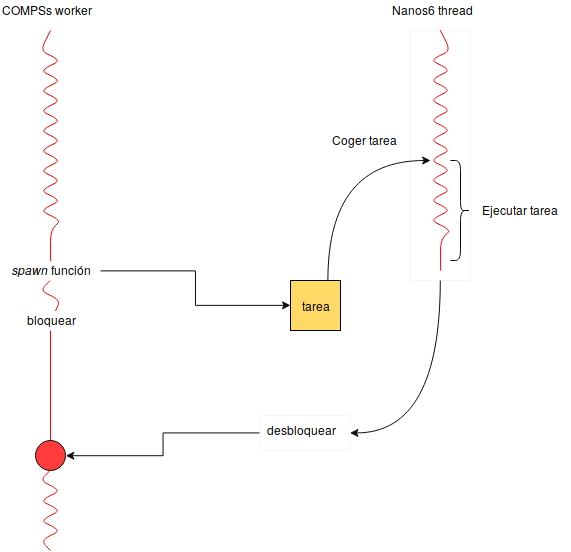
\includegraphics[scale=0.6]{spawn_sync.png}
    \label{fig:spawn_sync}
\end{figure}

En la figura anterior se muestran dos \textit{threads}, uno que registra una tarea y otro que espera a poder ejecutar alguna tarea. El primer \textit{thread} una vez haya registrado la tarea procederá a bloquearse, el segundo cuando acabe de ejecutar la tarea registrada, ejecutará un \textit{callback} donde desbloquearemos al primer \textit{thread}. \bigskip

El mecanismo abstracto es sencillo, pero la implementación real depende de los \textit{Pthreads}. Las estructuras utilizadas para realizar la sincronización son \texit{mutexes} y \textit{condition variables}. Un \textit{mutex} es una estructura que sirve para definir regiones de exclusión mútua mediante métodos de adquisición y liberación de la región, en este mecanismo se utilizan tan sólo por que son necesarios para utilizar \textit{condition variables}. Las \textit{condition variables} nos permiten que un \textit{thread} espere a un evento de manera no bloqueante, si no, habría que hacer \textit{polling} y consumir tiempo de cómputo inútilmente.
\bigskip

Será con las funciones \textit{pthread\_cond\_wait(pthread\_cond\_t * cond, pthread\_mutex\_t * mutex)} y \textit{pthread\_cond\_signal(pthread\_cond\_t * cond)} con las que respectivamente bloqueemos al primer \textit{thread} después de registrar la tarea y lo desbloqueemos al acabar de ejecutarla.
\bigskip

Dado que para utilizar \textit{condition variables} se necesitan \textit{mutexes} y se recomienda utilizar una variable auxiliar para evitar abrazos mortales (en el caso de que, el segundo \textit{thread} ya ha intentado desbloquear al primero, pero este aún no se había bloquedao, cuando se bloquee, se bloqueará para siempre), se crea una estructura de datos para contener todas estas variables llamada \textit{condition\_variable\_t}.

\smallskip

\begin{lstlisting} [caption={Definición de la estructura de datos condition\_variable\_t.},captionpos=b, label={lst:wait-condition}, language=C++]
typedef struct {
    pthread_mutex_t _mutex;
    pthread_cond_t _cond;
    int _signaled;
} condition_variable_t;
\end{lstlisting}

\smallskip

\begin{lstlisting} [caption={Función wait\_condition\_variable},captionpos=b, label={lst:wait-condition}, language=C++]
void wait_condition_variable(condition_variable_t *cond_var)
{
    pthread_mutex_lock(&cond_var->_mutex);
    while (cond_var->_signaled == 0) {
        pthread_cond_wait(&cond_var->_cond, &cond_var->_mutex);
    }
    pthread_mutex_unlock(&cond_var->_mutex);
}
\end{lstlisting}

En la imagen \ref{lst:library-main} se utiliza la función \textit{wait\_condition\_variable(&cond\_var)}, la llamada a  \textit{pthread\_cond\_wait} está dentro de una región crítica para prevenir que nadie más se bloquee sobre la misma \textit{condition variable} y esta se encuentra dentro de un \textit{while} por que puede ocurrir que el \textit{thread} se desbloquee sin haber sido desbloqueado por otro \textit{thread}, la variable \textit{cond\_var->\_signaled} será 0 hasta que el \textit{thread} que produzca el desbloqueo lo modifique, así garantizaremos que el desbloqueo es intencionado.
\smallskip

\begin{lstlisting} [caption={Callback de la tarea registrada},captionpos=b, label={lst:signal-condition}, language=C++]
void condition_variable_callback(void *untyped_arg)
{
    condition_variable_t *cond_var = (condition_variable_t *) untyped_arg;

    pthread_mutex_lock(&cond_var->_mutex);
    cond_var->_signaled = 1;
    pthread_cond_signal(&cond_var->_cond);
    pthread_mutex_unlock(&cond_var->_mutex);
}
\end{lstlisting}

La imagen anterior muestra el \textit{callback} que se ejecuta al finalizar la ejecución de la tarea, modifica el valor de la variable \textit{cond\_var->\_signaled} y efectúa un \textit{pthread\_cond\_signal} para despertar al primer \textit{thread}.













\section{Código para realizar la integración COMPSs+OmpSs-2}
\label{appendix:integration}

\subsection{Ejecutar tareas de COMPSs como tareas de OmpSs-2}

Para la implementación de los \textit{workers} hay dos ficheros distintos \textit{nio\_worker\_c.cc} y \textit{worker\_c.cc} respectivamente para el persistente y el no persistente. En cada uno de estos ficheros deberemos añadir el código para que cuando los compilemos con la opción de \textit{OmpSs-2} y \textit{COMPSs} los ejecute (en función de si es persistente o no) y activen el modo librería.

\bigskip

\begin{minipage}{\linewidth}
\begin{lstlisting} [caption={Código necesario para la gestión del modo librería de Nanos6 en nio\_worker\_c.cc y worker\_c.cc},captionpos=b, label={lst:managementnanosworkers}, language=C++]

#ifdef OMPSS2_ENABLED
#include <pthread.h>
#include <nanos6/bootstrap.h>
#include <nanos6/library-mode.h>
#endif

    ...

#ifdef OMPSS2_ENABLED
    char const *error = nanos6_library_mode_init();
    if (error != NULL)
    {
        fprintf(stderr, "Error initializing Nanos6: %s\n", error);
        return 1;
    }
    std::cout << "[C-BINDING] Nanos6 initialized" << std::endl;
#endif

    ...
    
#ifdef OMPSS2_ENABLED
    nanos6_shutdown();
    std::cout << "[C-BINDING] Nanos6 shutdown" << std::endl;
#endif

\end{lstlisting}
\end{minipage}

\par\bigskip

El código mostrado en la imagen \ref{lst:managementnanosworkers} se divide en tres bloques divididos por puntos suspensivos, el código que hubiera entre estos, depende de si el fichero es \textit{nio\_worker\_c.cc} o \textit{worker\_c.cc} y es independiente de ellos. Se hace uso de macros del preprocesador de \textit{C}, la macro \textit{\#ifdef VAR} comprueba en tiempo de compilación si la variable \textit{OMPSS2\_ENABLED} está definida, si lo está las líneas contenidas entre la primera y el \textit{\#endif} serán incluidas en el fichero, sino no lo serán.
\par\medskip
En cuánto a los tres bloques, el primero incluye cabeceras necesarias para \textit{Nanos6}, y el resto han sido ya explicados en la sección \ref{spawnfunction}.
\par\bigskip

En el caso de \textit{OmpSs}, hay que registrar exactamente los \textit{threads} de un proceso que ejecutarán tareas y también hay que compilar necesariamente toda la aplicación con \textit{Mercurium} y el \textit{flag} \textit{-{}-ompss}, pero por otra parte, no hay necesidad de añadir más código a parte del que se encarga de registrar los \textit{threads}. En \textit{OmpSs-2} como vimos en el ejemplo, es necesario hacer una gestión más compleja en cuánto a generación de código, pero es independiente del \textit{thread} en el cuál se ejecuta.
\par\bigskip
Con tal de cambiar el código que se genera en el \textit{executor}, hay que hacer modificaciones en el programa que compila la interfaz del programa para generar el \textit{stubs}, el \textit{executor} y el resto de ficheros necesarios. En la estructura que tenemos nosotros del compilador, el fichero que contiene el código para autogenerarlo todo es \textit{c-backend.c}, en el cuál deberemos hacer unas modificaciones.
\par\smallskip
Vamos a centrarnos en las modificaciones que harán que podamos generar el \textit{struct} personalizado para cada tarea y la llamada a \textit{nanos6\_spawn\_function}, pero cómo se genera el mecanismo de sincronización  (\textit{pthread\_cond\_wait}, \textit{pthread\_cond\_signal} y las estructuras de datos necesarias) es trivial, ya que no varía según la aplicación que se compile, es siempre el mismo.
\par\bigskip
Con tal de generar el \textit{struct} para cada tarea, incluiremos su definición en los ficheros que hacen la función de cabecera. Cada \textit{struct} será único para cada tarea (podría tener los mismos campos, pero nunca el mismo nombre). Para generar el \textit{struct} de la tarea, necesitamos tener información sobre la función que se ejecutará, contamos con una estructura \textit{function} que almacena toda la información necesaria.
\par\bigskip

La imagen \ref{lst:structs} contiene el código necesario para incluir en la cabecera la definición del \textit{struct} de una función en concreto. Se recorrerán los argumentos de la función y se comprobará si tiene retorno, habrá un campo del \textit{struct} por cada argumento que tenga la función y uno adicional en caso de que tenga retorno.

\bigskip

\begin{minipage}{\linewidth}
\begin{lstlisting} [caption={Función para generar la definición de los structs.},captionpos=b, label={lst:structs}, language=C++]
static void generate_struct_nanos6_wrapper(FILE *outFile, 
Types current_types,
function *func) {
argument *arg;
fprintf(outFile, "typedef struct {\n", func->methodname);

char* return_type = construct_returntype(func);

if (func->return_type != void_dt && return_type != NULL) {
fprintf(outFile, "\t% s ret;\n", return_type);
}

arg = func->first_argument;
while (arg != NULL) {
fprintf(outFile, "\t% s;\n", construct_type_and_name(arg));
arg = arg->next_argument;
}
fprintf(outFile, "} % s_struct_t;\n", func->methodname);
}
\end{lstlisting}
\end{minipage}

\par\bigskip
Para generar el código del \textit{wrapper} lo primero que necesitamos hacer es generar el nombre de la función, que es del estilo ''function\_wrapper'' y tiene por argumento un puntero a \textit{void} que apunta al \textit{struct} que contiene los argumentos para la función que vamos a ejecutar y el valor de retorno de esta en caso que tenga. Entonces, si la función tiene retorno distinto del tipo \textit{void}, la ejecutaremos asignándole el valor al \textit{struct}, en caso contrario tan sólo la ejecutaremos, si algún valor de los argumentos se modifica, la única posibilidad para que esto se refleje en \textit{COMPSs} es que fuera un puntero, por lo que quedará modificado también dentro del \textit{struct}.

\smallskip
La imagen \ref{lst:wrapper} muestra como está hecho.
\bigskip

%\begin{minipage}{\linewidth}
\begin{lstlisting} [caption={Función para generar el wrapper de la tarea.},captionpos=b, label={lst:wrapper}, language=C++]

static void generate_nanos6_wrapper(FILE *outFile, function* func) {
fprintf(outFile, "void % s_wrapper(void* args) {\n", 
func->methodname);

fprintf(outFile, 
"\t% s_struct_t* struct_ = (% s_struct_t*) args;\n", 
func->methodname, 
func->methodname);

char* func_to_execute;
int printed_chars = 0;

if (func->return_type != NULL && func->return_type != void_dt) {
fprintf(outFile, "\tstruct_->ret = ", func->return_type);
}

if ((func->classname != NULL) && (func->access_static == 0)) {
printed_chars = asprintf(&func_to_execute, 
"\t% s->% s(", 
func->name, 
func->methodname);
} else {
printed_chars = asprintf(&func_to_execute, 
"\t% s(", func->name);
}

if (printed_chars < 0) {
asprintf_error(func_to_execute, 
"ERROR: Not possible to 
generate method execution.\n");
}

fprintf(outFile, "% s", func_to_execute);

argument* args = func->first_argument;

int first = 1;
while (args != NULL) {
if (first) {
first = 0;
}
else {
fprintf(outFile, ", ");
}
fprintf(outFile, "struct_->% s", args->name);

args = args->next_argument;
}

fprintf(outFile, ");\n");
fprintf(outFile, "}\n");
}  
\end{lstlisting}
%end{minipage}
\par\bigskip

Ahora ya tenemos lo que necesitamos, \textit{structs} para pasar los argumentos, el \textit{wrapper} del que haremos \textit{spawn} y la propia tarea que se acabará ejecutando, tan sólo falta hacer la llamada a \textit{nanos6\_spawn\_function}. Para hacer esto, tenemos que declarar el \textit{struct} y asignarle los valores que vienen de \textit{COMPSs}, acto seguido se generará la llamada a \textit{nanos6\_spawn\_function} con el \textit{wrapper} como función a ejecutar desde \textit{OmpSs-2}, la dirección del \textit{struct} que contiene los argumentos y todo lo necesario para efectuar los mecanismos de sincronización que vimos en la sección \ref{sec:mecanismosync}. Una vez hemos esperado a que la tarea se haya ejecutado, si el retorno era distinto del tipo \textit{void} hay que asignarlo al retorno de la tarea a nivel de \textit{COMPSs}. En la imagen \ref{lst:spawncompss} se ve el código que se encarga de generar esta parte.
\bigskip

\begin{minipage}{\linewidth}
\begin{lstlisting} [caption={Código para hacer un spawn de una tarea para OmpSs-2 en COMPSs.},captionpos=b, label={lst:spawncompss}, language=C++]
fprintf(outFile, "\t\t\t% s_struct_t % s_struct;\n", func->methodname, 
func->methodname);

assign_arguments_to_struct(outFile, func);

char* nanos6_spawner;
printed_chars = asprintf(&nanos6_spawner, 
"\t\t\tnanos6_spawn_function(% s_wrapper,
&% s_struct, 
% s, % s, 
\"% s_spawned_task\");\n",
func->methodname, 
func->methodname, 
"condition_variable_callback", 
"&cond_var", 
func->methodname);

if (printed_chars < 0) {
asprintf_error(nanos6_spawner, 
"Not possible to generate function spawn.\n");
}

fprintf(outFile, "% s\n", nanos6_spawner);

fprintf(outFile, "\t\t\twait_condition_variable(&cond_var);\n");

if (func->return_type != void_dt && func->return_type != NULL) {
char* return_var;
printed_chars = asprintf(&return_var, 
"return_obj = % s_struct.ret;\n", 
func->methodname);

fprintf(outFile, "% s", return_var);

if (printed_chars < 0) {
asprintf_error(return_var, 
"Not possible to generate return variable.\n");
}
}
\end{lstlisting}
\end{minipage}

\bigskip
\subsection{Entorno de compilado para aplicaciones COMPSs+OmpSs-2}

Para compilar una aplicación que utilice \textit{OmpSs} se necesita poner el \textit{flag} \textit{-{}-ompss} en \textit{Mercurium}, y el \textit{flag} \textit{-{}-ompss-2} para \textit{OmpSs-2}. En la anterior integración se compilaba la totalidad de los ficheros con \textit{Mercurium} y el \textit{flag} \textit{-{}-ompss} debido a que no existía el modo librería. Ahora, es estrictamente necesario compilar con \textit{Mercurium} y el \textit{flag} \textit{-{}-ompss-2} tan sólo un único fichero, el que contiene las funciones a ejecutar como tareas. 
\par\bigskip
Habrá que modificar el método actual de compilación de una aplicación del \textit{binding} de \textit{C/C++} con tal de que aplique lo relativo a la compilación explicado en la sección \ref{sec:compilado}.
\par\bigskip

Para el usuario compilar una aplicación con \textit{OmpSs} es muy sencillo, ejecutando en el terminal el comando \textit{compss\_build\_app -{}-ompss ejemplo} empezaría el proceso de compilado del \textit{master} y el \textit{worker} de manera automática, en la nueva integración no puede ser más difícil. Antes de indagar en las modificaciones en concreto en los \textit{scripts} vamos a ver una descripción superficial de cómo se hace actualmente.

\bigskip
\begin{figure}[H]
	\centering 
	\caption{Estructura superficial de los \textit{scripts} para compilar una aplicación de COMPSs.}
	%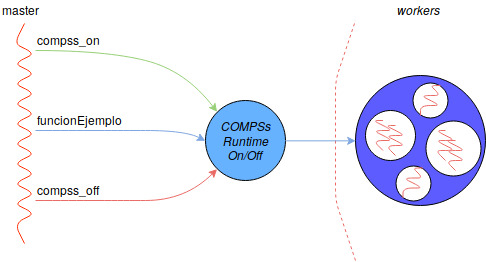
\includegraphics[width=\textwidth]{sta-masterworker.jpg}
	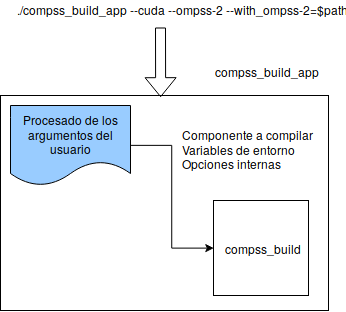
\includegraphics[scale=0.7]{compilation.png}
	\label{fig:compilado}
\end{figure}
\par\bigskip

En la imagen \ref{fig:compilado} vemos que existen dos \textit{scripts}, \textit{compss\_build\_app} y \textit{compss\_build}, el primero es el encargado de recoger los argumentos que el usuario haya introducido para la compilación de su aplicación (si se utiliza \textit{OmpSs}, donde está la instalación de \textit{OmpSs}, si se utiliza \textit{OpenCL}, o \textit{Cuda}, etc) y procesarlos configurando el entorno correcto para la compilación según estos argumentos que ha introducido el usuario. Una vez configurado el entorno se ejecuta el segundo \textit{script} \textit{compss\_build} tanto para el \textit{master} como para el \textit{worker}, que será realmente quién efectúe la compilación. 
\par\bigskip
Para ello se utiliza un conjunto de herramientas muy populares desarrolladas por \textit{GNU},  \textit{Autotools} \ref{appendix:autotools}. Estas herramientas tienen como objetivo facilitar a los usuarios (que no a los desarrolladores...) la compilación y portabilidad entre plataformas. Pese a que es un campo interesante y muy útil, no entraremos demasiado en detalles, daremos una visión general y entraremos en las modificaciones que se han realizado con tal de poder compilar aplicaciones del tipo \textit{COMPSs+OmpSs-2}. 
\par\bigskip
Como ya hemos visto, \textit{compss\_build\_app} hace de alguna manera de \textit{wrapper} de \textit{compss\_build}, es decir, lo ejecuta con los parámetros adecuados las veces que sea necesario. Este segundo, es el que toca de primera mano \textit{Autotools}, con tal de utilizarlo para compilar una aplicación hay que generar una serie de ficheros. La siguiente imagen nos muestra una porción del \textit{script}  \textit{compss\_build} para generar el \textit{script} \textit{autogen.sh}, que al ser ejecutado nos generará estos ficheros que \textit{Autotools} necesita.
\bigskip

\begin{minipage}{\linewidth}
\begin{lstlisting} [caption={Porción del script autogen.sh que genera los ficheros base necesarios para Autotools.},captionpos=b, label={lst:aclocal}, language=bash]
/bin/cat > autogen.sh << EOF
#!/bin/bash
set -e

/usr/bin/aclocal
/usr/bin/automake -a -c
/usr/bin/autoconf
EOF       
\end{lstlisting}
\end{minipage}

\par\bigskip

La primera y la última línea de la imagen \ref{lst:aclocal} sirven para escribir el código contenido entre estas en el fichero \textit{autogen.sh}. El \textit{script} \textit{autogen.sh} es generado por \textit{compss\_build} cada vez que se quiere compilar una aplicación y también en función de si se está compilando el \textit{master} o el \textit{worker} (de hecho, se encuentran en sitios distintos), tendrá una forma u otra. 
\par\smallskip

Una vez ejecutada esta porción del \textit{script} \textit{autogen.sh}, entre otros, esto nos habrá generado un \textit{script} \textit{configure}, que al ser ejecutado generará un \textit{Makefile} adaptado al entorno que hayamos especificado. Nuestro proceso de compilado requiere ser flexible, ya que permitimos utilizar \textit{OmpSs}, a veces con \textit{Cuda}, a veces con \textit{OpenCL}... Por tanto, necesitamos pasarle al compilador dónde se encuentran las librerías que necesitamos, \textit{flags} adicionales que necesitemos (\textit{-{}-ompss}, \textit{-{}-ompss-2}, \textit{-{}-cuda}...). Por suerte, este \textit{configure}, nos permite pasar variables de entorno a tener en cuenta durante la compilación, además de opciones personalizadas, a continuación del código de la imagen \ref{lst:aclocal} añadiremos código para que \textit{autogen.sh} ejecute el \textit{script} \textit{configure} con las opciones que necesitamos.
\bigskip

\begin{minipage}{\linewidth}
\begin{lstlisting} [caption={Porción del script autogen.sh que se encarga de customizar la ejecución de configure.},captionpos=b, label={lst:customconfigure}, language=bash]                                                                                                                                               
if [ "$OMPSS2_ENABLED" == "enabled" ]; then
ldflags_aux="$ldflags_aux -L$OMPSS2_DIR/lib
-Wl,-rpath,$OMPSS2_DIR/lib"
cflags_aux="$cflags_aux -I$OMPSS2_DIR/include"
conf_opts="--with-ompss-2"
fi

if [ "$OMPSS_ENABLED" == "enabled" ]; then
ldflags_aux="$ldflags_aux -L$OMPSS_DIR/lib"
cflags_aux="$cflags_aux -I$OMPSS_DIR/include"
conf_opts="$conf_opts --with-ompss"
fi

if [ "$CUDA_ENABLED" == "enabled" ]; then
ldflags_aux="$ldflags_aux -L$CUDA_HOME/lib64"
cflags_aux="$cflags_aux -I$CUDA_HOME/include"
conf_opts="$conf_opts --with-cuda"
fi

/bin/cat >> autogen.sh << EOF
./configure --with-cs-prefix=$CS_HOME $conf_opts \ 
CXXFLAGS="$CXXFLAGS $cflags_aux"     \  
CFLAGS="$CFLAGS $cflags_aux"         \
LDFLAGS="$LDFLAGS $ldflags_aux" 
EOF

/bin/chmod +x autogen.sh
\end{lstlisting}
\end{minipage}
\par\bigskip

Anteriormente hemos mencionado que el \textit{script} \textit{compss\_build\_app} es el encargado de recolectar los \textit{flags} que nos interesan del usuario en el proceso de compilación y servirlos al \textit{script} \textit{compss\_build}, como se puede ver en la imagen \ref{lst:customconfigure} en función de si las variables de entorno \textit{OMPSS2\_ENABLED}, \textit{OMPSS\_ENABLED}, o \textit{CUDA\_ENABLED} tienen por valor la cadena de carácteres \textit{enabled}, definirá el valor de los \textit{flags} para la fase de compilación \textit{CXXFLAGS} y \textit{CFLAGS}, que se asignarán via la variable \textit{cflags\_aux} y para la fase de \textit{linking} \textit{LDFLAGS} que se asignará via la variable \textit{ldflags\_aux}, además de las opciones personalizadas (que serán pasadas mediante la variable \textit{conf\_opts}).
\par\smallskip
Dos ficheros esenciales en todo este proceso, son \textit{configure.ac} y \textit{Makefile.am}, uno utiliza una serie de \textit{macros} para generar de manera customizada \textit{configure} (por ejemplo, con las opciones mencionadas anteriormente), y el otro indica cuáles son los ficheros que deben ser compilados, cómo y adónde irán una vez compilados.
\par\bigskip
Las modificaciones que explicamos ahora mismo sólo se han aplicado al \textit{worker}, para el \textit{master} no se ha necesitado ningún tipo de modificación. Para declarar una opción personalizada en \textit{configure} se utiliza la macro \textit{AC\_ARG\_WITH}, que tiene como argumentos el nombre de la opción (ompss, que pasará a ser with-ompss), el mensaje de ayuda para el usuario y lo que hay que hacer en caso que se habilite la opción, la imagen \ref{lst:ac-ompss} muestra exactamente cómo se hace.

\bigskip

\begin{minipage}{\linewidth}
\begin{lstlisting} [caption={Macros necesarias en configure.ac para habilitar la opcion --ompss en configure.},captionpos=b, label={lst:ac-ompss}, language=bash]
AC_ARG_WITH([ompss],
AS_HELP_STRING([ --with-ompss], [Enables the use of OmpSs and 
specificates its directory.]),
[
ompss=true
]
)
\end{lstlisting}
\end{minipage}

\par\bigskip

Para el resto de opciones se utiliza el mismo mecanismo, pero las acciones a realizar si se habilita la opción son distintas. Con tal de compilar una aplicación de \textit{OmpSs-2} necesitamos librerías de \textit{Pthreads}, \textit{dl}\footnote{https://en.wikipedia.org/wiki/Dynamic\_loading}, \textit{nanos6} (evidentemente para todo lo que concierne al \textit{runtime}), y \textit{custom-nanos6}, que no es más que la adaptación a librería del \textit{nanos6-library-mode.o} que se utilizó en la sección \ref{sec:compilado}. La imagen \ref{lst:ac-ompss-2} muestra exactamente cómo lo hacemos.

\bigskip

\begin{minipage}{\linewidth}
\begin{lstlisting} [caption={Macros necesarias en configure.ac para habilitar la opcion --ompss-2 en configure.},captionpos=b, label={lst:ac-ompss-2}, language=bash]
AC_ARG_WITH([ompss-2],
AS_HELP_STRING([ --with-ompss-2], [Enables the use of OmpSs2 
and specificates its 
directory.]),
[
ompss2=true

AC_CHECK_LIB([pthread], 
[pthread_cond_signal], 
[],
[
AC_MSG_ERROR([Pthread library not found, 
is needed to enable OmpSs2.])
])

AC_CHECK_LIB([dl], 
[dlopen], 
[],
[
AC_MSG_ERROR([dl library not found, 
is needed to enable OmpSs2.])
])

AC_CHECK_LIB([nanos6], 
[nanos6_spawn_function], 
[],
[
AC_MSG_ERROR([Nanos6 library not found, 
is needed to enable OmpSs2.])
])

AC_CHECK_LIB([custom-nanos6], 
[nanos6_library_mode_init], 
[],
[
AC_MSG_ERROR([nanos6-library-mode.o is needed, 
we make a custom library from it.])
])
]
)
\end{lstlisting}
\end{minipage}

\par\bigskip

En este caso a parte de la macro \textit{AC\_ARG\_WITH} se utiliza \textit{AC\_CHECK\_LIB}, esta macro hará que se compruebe si la librería del primer argumento existe y contiene la función del segundo argumento, el tercer y el cuarto argumento indican respectivamente que se hará si se encuentra la librería y que se hará en caso que no se encuentre. Nótese que esta macro, añade la librería a la variable de entorno \textit{LIBS} (librerías que tomarán parte en la fase de \textit{linking}). En el caso de cuda debemos buscar la librería del \textit{runtime} de \textit{Cuda}, que es \textit{cudart}. Se utilizan exactamente los mismos mecanismos que en el resto de opciones, se muestra exactamente en la imagen \ref{lst:ac-cuda}.

\bigskip

\begin{minipage}{\linewidth}
\begin{lstlisting} [caption={Macros necesarias en configure.ac para habilitar la opcion --cuda en configure.},captionpos=b, label={lst:ac-cuda}, language=bash]
AC_ARG_WITH([cuda],
AS_HELP_STRING([ --with-cuda], [Enables the use of CUDA.]),
[
cuda=true

AC_CHECK_LIB([cudart], 
[cudaMalloc], 
[],
[
AC_MSG_ERROR([cudart library not found, 
is needed to enable CUDA.])
])
]
)
\end{lstlisting}
\end{minipage}

\par\bigskip

Para todas las opciones, en las imágenes \ref{lst:ac-ompss}, \ref{lst:ac-ompss-2} y \ref{lst:ac-cuda} se asigna el valor a una variable ompss, ompss-2 y cuda respectivamente para cada opción al valor \textit{true}. Con la macro \textit{AC\_CONDITIONAL} asignamos a una variable con el nombre del primer argumento el valor que obtengamos del segundo. Estas variables son visibles en el fichero \textit{Makefile.am}, de manera que podremos condicionar la compilación en función de que opciones pase el usuario al \textit{script} \textit{configure}.

\par\bigskip

\begin{minipage}{\linewidth}
\begin{lstlisting} [caption={Creación de las variables para el Makefile.am.},captionpos=b, label={lst:ac-vars}, language=bash]
AM_CONDITIONAL([OMPSS]      , [test x$ompss = xtrue])
AM_CONDITIONAL([OMPSS2]     , [test x$ompss2 = xtrue])
AM_CONDITIONAL([CUDAOMPSS]  , [test x$cuda = xtrue && 
test x$ompss = xtrue])
AM_CONDITIONAL([CUDAOMPSS2] , [test x$cuda = xtrue && 
test x$ompss2 = xtrue])
\end{lstlisting}
\end{minipage}

\par\bigskip

Esto sería todo lo relacionado con el \textit{configure.ac}, ahora entraríamos con el \textit{Makefile.am}. Recordemos que lo único que necesitamos compilar con \textit{-{}-ompss-2} es el fichero que contiene las funciones a ser ejecutadas como tareas, por lo tanto necesitamos hacer una distinción de los \textit{flags} que se utilizan para compilar este fichero. Para conseguir esto, hemos decidido indicar en el \textit{Makefile.am} que se haga una librería de este fichero y se compile con unos \textit{flags} en especial, para así aislarlo del resto. En la siguiente imagen se muestra como se hace esto.

\par\bigskip

La primera línea indica que \textit{libfunctions.a} es una librería que no debe ser instalada, y la segunda que el fichero fuente de esta librería es \textit{PACKAGE-functions.cc} donde \textit{PACKAGE} es el nombre del paquete. Las siguientes líneas indican los \textit{flags} base que se utilizarán para compilar los ficheros fuente.
 
\bigskip

\begin{minipage}{\linewidth}
\begin{lstlisting} [caption={Crear una librería en el Makefile.am.},captionpos=b, label={lst:am-lib}, language=bash]
noinst_LIBRARIES = libfunctions.a
libfunctions_a_SOURCES = PACKAGE-functions.cc

libfunctions_a_CPPFLAGS =  -I../../src -I../../include
-Wno-write-strings -I$(JAVA_HOME)/include 
-I$(JAVA_HOME)/include/linux/ -Wall
-I$(CS_HOME)/../bindings-common/include
-I$(CS_HOME)/include 

libfunctions_a_CFLAGS =
\end{lstlisting}
\end{minipage}

\par\bigskip
A esta altura, ya tenemos la base para compilar la librería, pero si no podemos poner los \textit{flags} para \textit{OmpSs-2} o \textit{OmpSs} no habremos conseguido nada. Utilizaremos las variables que hemos definido anteriormente en \ref{lst:ac-vars}. Sencillamente, en función de si las variables correspondientes tienen el valor adecuado, añadimos a las variables adecuadas los \textit{flags} que requerimos. Por ejemplo, si el usuario está compilando con \textit{OmpSs-2}, los \textit{flags} para compilar \textit{libfunctions.a} deben contener \textit{-{}-ompss-2} entre otros. En la imagen \ref{lst:am-cond-flags} se procede a asignar los \textit{flags} de esta manera.
\bigskip

\begin{minipage}{\linewidth}
\begin{lstlisting} [caption={Flags de manera condicional en Makefile.am.},captionpos=b, label={lst:am-cond-flags}, language=bash]
if OMPSS2
libfunctions_a_CPPFLAGS  += --ompss-2 -DOMPSS2_ENABLED
libfunctions_a_CFLAGS    += --ompss-2 -DOMPSS2_ENABLED

nio_worker_c_CPPFLAGS    += -DOMPSS2_ENABLED
worker_c_CPPFLAGS        += -DOMPSS2_ENABLED
endif

if OMPSS
libfunctions_a_CPPFLAGS  += --ompss -DOMPSS_ENABLED
libfunctions_a_CFLAGS    += --ompss -DOMPSS_ENABLED

nio_worker_c_CPPFLAGS    += --ompss -DOMPSS_ENABLED
worker_c_CPPFLAGS        += --ompss -DOMPSS_ENABLED

nio_worker_c_LDFLAGS += --ompss
worker_c_LDFLAGS     += --ompss
endif

if CUDAOMPSS
libfunctions_a_CPPFLAGS  += --cuda -DCUDA_ENABLED
libfunctions_a_CFLAGS    += --cuda -DCUDA_ENABLED

nio_worker_c_CPPFLAGS    += --cuda -DCUDA_ENABLED
worker_c_CPPFLAGS        += --cuda -DCUDA_ENABLED

nio_worker_c_LDFLAGS += --cuda
worker_c_LDFLAGS     += --cuda
endif

if CUDAOMPSS2
libfunctions_a_CPPFLAGS  += --cuda -DCUDA_ENABLED
libfunctions_a_CFLAGS    += --cuda -DCUDA_ENABLED
endif
\end{lstlisting}
\end{minipage}

\par\bigskip
Está claro que después de haber compilado la librería habrá que hacer el \textit{linking} de ella con \textit{nio\_worker\_c} o \textit{worker\_c}. Con esto ya habríamos hecho las modificaciones necesarias para poder compilar la aplicación de \textit{COMPSs+OmpSs-2}.

\subsection{Soporte para el tipo enum y cabeceras en la interfaz}

Un requisito ha sido soportar el tipo \textit{enum} y añadir la posibilidad de incluir cabeceras en la interfaz de una aplicación \textit{C/C++}. Para hacer esto, ha habido que hacer modificaciones en la gramática del compilador y en la generación de código. Este añadido puede ser muy útil para cuando se utilicen librerías externas en la interfaz y se precise de cabeceras adicionales que incluyan tipos que se necesitan.
\par\bigskip
El compilador está hecho con las herramientas \textit{Lex} (un generador de analizadores léxicos) y \textit{Yacc} (un generador de analizadores sintácticos), es decir, las dos piezas fundamentales para hacer un compilador, ya que uno nos facilitará el reconocimiento de \textit{tokens} en la interfaz y el otro nos permite comprobar que realmente tiene sentido la interfaz y le otorga una semántica.
\par\bigskip
Para añadir el tipo \textit{enum}, la gramática tiene que reconocer algo del estilo "\textit{in/out enum} tipo nombre\_variable" y asociarle el comportamiento que el compilador tiene con el tipo entero al del \textit{enum} ya que al final ambos son enteros. De forma similar, para el \textit{include} hubo modificar la gramática para que reconociera el patrón "\textit{include} nombre\_cabecera;" y al generar el código incluir la cabecera.
\par\bigskip

En cuánto las modificaciones a hacer en \textit{Lex} son relativas a los \textit{tokens} que el analizador deberá detectar, la siguiente imagen muestra las modificaciones.
\bigskip

\begin{minipage}{\linewidth}
\begin{lstlisting} [caption={Porción del analizador sintáctico para soportar tipo enum y interface.},captionpos=b, label={lst:lex-tok-enum-interface}, language=C++]
...
header_identfier [a-zA-Z][0-9a-zA-Z_]*\.[a-z]*
%%
...
enum        return TOK_ENUM;
include     return TOK_INCLUDE;
{header_identfier} yylval.name = strdup(yytext); return TOK_HEADER;
%%
\end{lstlisting}
\end{minipage}

\par\bigskip
Se define \textit{header\_identifier} como una expresión regular que identificará correctamente cualquier cabecera del estilo que hemos dicho antes. A continuación se define qué \textit{token} devolverán \textit{enum} \textit{include} y \textit{header\_identifier}. Ahora podremos utilizar esto en \textit{Yacc}.

\par\bigskip
La siguiente imagen muestra todas las modificaciones hechas en la gramática para dar el soporte. Básicamente se añaden a una estructura de datos el \textit{TOK\_HEADER} (\textit{include}) y el \textit{enum\_type} que es una regla definida por el \textit{token} \textit{TOK\_ENUM} (\textit{enum}), se crea la regla \textit{includes} con las características descritas y ejecuta la función entre llaves \textit{add\_header}, además se añade otra regla nueva a \textit{argument}, que son todos los posibles aspectos (tipo, dirección...) que argumento puede tener en una tarea. Esta nueva regla reconoce una dirección (entrada o salida), un \textit{enum\_type}, y dos \textit{TOKEN\_IDENTIFIER} que corresponden con el nombre del \textit{enum}, es decir el tipo en sí, y el nombre del argumento. Una vez reconocido este patrón se ejecuta la función entre llaves \textit{add\_argument}.
\bigskip

\begin{minipage}{\linewidth}
\begin{lstlisting} [caption={Porción de la gramática para soportar tipo enum y interface.},captionpos=b, label={lst:gram-tok-enum-interface}, style=YStyle]
% union {
char        *elements;
char        *name;
char        *classname;
enum datatype   dtype;
enum direction  dir;
}
... 
% token TOK_ENUM TOK_HEADER

% token <name> TOK_IDENTIFIER TOK_HEADER
% token <elements> NUMBER
% type <dtype> data_type numeric_type array_type enum_type
% type <dir> direction
...
%%
enum_type: TOK_ENUM { $$ = enum_dt; }
;
...
includes: 
| includes TOK_INCLUDE TOK_HEADER { add_header($3); } TOK_SEMICOLON
;

argument:   direction data_type TOK_IDENTIFIER { add_argument($1, $2, "", $3, NULL); }

|   direction array_type TOK_LEFT_BRAKET TOK_IDENTIFIER TOK_RIGHT_BRAKET TOK_IDENTIFIER 
											   { add_argument($1, $2, "", $6, $4);}
											   
|   direction array_type TOK_LEFT_BRAKET NUMBER TOK_RIGHT_BRAKET TOK_IDENTIFIER 
											   { add_argument($1, $2, "", $6, $4);}
											   
|   direction TOK_IDENTIFIER TOK_IDENTIFIER 
											   { add_argument($1, object_dt, $2, $3, NULL); }
											   
|   direction enum_type TOK_IDENTIFIER TOK_IDENTIFIER 
											   { add_argument($1, $2, $3, $4, NULL); }
;
%%
...
\end{lstlisting}
\end{minipage}

\par\bigskip
Con el fragmento de la imagen \ref{lst:gram-tok-enum-interface} y el resto del código que no aparece, \textit{Yacc} generará un fichero \textit{C} que es la implementación del analizador sintáctico. 
\par\bigskip

Las funciones \textit{add\_header} y \textit{add\_argument} están implementadas en C (junto a otras muchas funciones que no veremos), y hacen uso de estructuras de datos que se utilizarán luego al generar el código, la fase que estamos viendo nos permite crear estructuras de datos que representen correctamente la interfaz y serán las que determinen en el paso de generar el código cómo queda este. La imagen \ref{lst:semantic} contiene la definición de las estructuras de dato que se irán repitiendo en lo queda de sección.

\bigskip
\begin{minipage}{\linewidth}
\begin{lstlisting}[caption={Definición de las estructuras de datos utilizadas en el compilador.},captionpos=b, label={lst:semantic}, language=C++]
struct argument {
char *name;
char *classname;
enum datatype   type;
enum direction  dir;
enum stream     stream;
int passing_in_order;
int passing_out_order;
char *elements;
argument *next_argument;
};

struct constraint {
char *name;
constraint *next_constraint;
};

struct include {
char *name; //Name of the header to include
include *next_include;
};

struct function {
char *name;
int access_static;
char *methodname;
char *classname;
char *return_typename;
enum datatype return_type;
char *return_elements;
argument *first_argument;
int argument_count;
int exec_arg_count;
constraint *first_constraint;
function *next_function;
};

struct interface {
char *name;
function *first_function;
};
\end{lstlisting}
\end{minipage}

\par\bigskip

Cuando se llama a \textit{add\_header} en \ref{lst:gram-tok-enum-interface} se le pasa el nombre de la cabecera a incluir, si es la primera vez que se ha incluido una cabecera en la interfaz habrá que asignar memoria para la variable \textit{current\_include} del tipo \textit{include} y asignarle el nombre de la cabecera. En caso que no fuera la primera vez, se encadenaría la nueva inclusión a la estructura \textit{include} actual en el campo \textit{next\_include}. De esta manera tendríamos siempre un puntero a la primera cabecera y en caso de haber más se apuntarían una detrás de otra. La imagen \ref{lst:addheader} contiene el código de la función \textit{add\_header}.

\bigskip

\begin{minipage}{\linewidth}
\begin{lstlisting} [caption={Función add\_header.},captionpos=b, label={lst:addheader}, language=C++]
void add_header(char* name) {
	debug_printf("Adding header %s\n", name);

	if (current_include == NULL) {
		current_include = (include*) malloc(sizeof(include));
	}
	else {
		current_include->next_include = (include*) malloc(sizeof(include));
		current_include = current_include->next_include;
	}
	current_include->name = name;

	if (first_include == NULL) {
		first_include = current_include;
	}
}
\end{lstlisting}
\end{minipage}

\bigskip
Cada vez que se reconoce un argumento se ejecuta la función \textit{add\_argument}, que se encargará de crear las estructuras \textit{argument} y añadirlas a la estructura \textit{current\_function}, que es la función que está siendo procesada actualmente, así cuando se hayan procesado todos los argumentos de la función actual está tendrá punteros a todas las estructuras que representan sus argumentos. En la imagen \ref{lst:addargument} se han omitido partes del \textit{switch} que correspondían a otros tipos de dato, en cualquier caso el código que se muestra basta para saber cómo se hace con el tipo \textit{enum}. 
 \bigskip

\begin{minipage}{\linewidth}
\begin{lstlisting} [caption={Función add\_argument.},captionpos=b, label={lst:addargument}, style=YStyle]
void add_argument(enum direction dir, enum datatype dt, char *classname, char *name, char* elements) {
	argument *new_argument;
	debug_printf("Add argument %i %i %s %s %s \n", dir, dt, classname, name, elements);
	assert(current_function != NULL);
	if (exists_argument(name)) {
		fprintf(stderr, "%s:%i: Duplicated argument name '%s' in function '%s'\n",
		get_filename(), line, name, get_current_function_name());
		has_errors = 1;
		return;
	}
	if (dt == void_dt) {
		fprintf(stderr, "%s:%i: Invalid parameter type for argument %i in function '%s'\n",
		get_filename(), line, get_next_argnum(), get_current_function_name());
		has_errors = 1;
		return;
	}
	new_argument = (argument *)malloc(sizeof(argument));
	new_argument->name = strdup(name);

    switch (dt) {
    
    ...
    
    case enum_dt:
    	new_argument->elements = "0";
    	new_argument->type = enum_dt;
    	new_argument->classname = strdup(classname);
    	break;
    
    ...
    
    }
    
    new_argument->dir = dir;
    new_argument->passing_in_order = 0;
    new_argument->passing_out_order = 0;
    new_argument->next_argument = NULL;
    
    if (current_argument != NULL) {
    	current_argument->next_argument = new_argument;
    } 
    else {
    	current_function->first_argument = new_argument;
    }
    current_argument = new_argument;
    current_function->argument_count++;
    
    switch (dir) {
    case in_dir:
    case out_dir:
    	current_function->exec_arg_count++;
    	break;
    case inout_dir:
    	current_function->exec_arg_count += 2;
    	break;
    default:
    	break;
    }
}
\end{lstlisting}
\end{minipage}

\par\bigskip
Ahora cuando vayamos a generar código ya tendremos en cuenta el \textit{enum} y el añadido de cabeceras. El \textit{enum} se trata igual que el \textit{int}, pero para el caso de las cabeceras se ha tenido que añadir una nueva función a la generación de código. 
\bigskip

%\begin{minipage}{\linewidth}
\begin{lstlisting} [caption={Funciones para incluir las cabeceras.},captionpos=b, label={lst:genheader}, language=C++]
static void include_header(include* current_include) {
	fprintf(includeFile, "#include <%s>\n", current_include->name);
}

static void add_include_headers(include* first_include) {
	include* include = first_include;

	while (include != NULL) {
		include_header(first_include);
		include = include->next_include;
	}
}
\end{lstlisting}
%\end{minipage}

\par\bigskip
En la imagen \ref{lst:genheader} están las funciones \textit{include\_header} y \textit{add\_include\_headers}, la primera dada una estructura \textit{include} que contiene el nombre de la cabecera a incluir imprime en el \textit{includeFile} la macro para incluirla, y la segunda dado el primer \textit{include} los recorre e incluye todos.
\newpage

%https://www.gnu.org/software/automake/manual/html_node/Autotools-Introduction.html

\section{Autotools}
\label{appendix:autotools}
 
\textit{Autotools} es un conjunto de herramientas que pretenden facilitar la difícil tarea de crear codigo fuente portable entre plataformas del tipo \textit{UNIX} de manera sencilla, es decir, de poder compilar el código fuente de una aplicación en en varias plataformas implicando un esfuerzo pequeño (para el usuario). \textit{Autotools} forma parte de la \textit{GNU Toolchain} desarrollado por el \textit{GNU Project\footnote{https://www.gnu.org/gnu/thegnuproject.html}}.

\newpage

\section{Estudio previo del rendimiento: código del test}
\label{appendix:estudioprevio}

\begin{minipage}{\linewidth}
\begin{lstlisting} [caption={Programa principal del test},captionpos=b, 
label={lst:tltmain}, language=C++]
#include <iostream>
#include <c_compss.h>
#include "tlt.h"
using namespace std;

int main() {
	cout << "Encendemos el runtime... " << endl;

	compss_on();
	
	int* array_a = (int*) malloc(30 * sizeof(int));
	int* array_b = (int*) malloc(30 * sizeof(int));
	
	for (int i = 0; i < 30; ++i) {
	
		coarse_task(array_a, 30);
		
		fine_task(array_b, 30);
	
	}
	
	compss_wait_on(array_a);
	compss_wait_on(array_b);   
		
	cout << "Apagamos el runtime... "   << endl;
	compss_off();

}   
\end{lstlisting}
\end{minipage}

\begin{minipage}{\linewidth}
\begin{lstlisting} [caption={Interfaz de la aplicación de test},captionpos=b, 
label={lst:idltlt}, style=idlstyle] 
interface tlt {

void coarse_task(inout int[N] a, in int N);

void fine_task(inout int[N] a, in int N);

};
\end{lstlisting}
\end{minipage}

\begin{minipage}{\linewidth}
\begin{lstlisting} [caption={Funciones a ejecutar como tareas del test},captionpos=b,
label={lst:tltfuncs}, language=C++] 
#include <unistd.h>
#include <stdio.h>

#define COARSE_GRAIN_SLEEP 300000
#define FINE_GRAIN_SLEEP 50000

void coarse_task(int* a, int N) {
	
	int i;
	for (i = 0; i < N; ++i) {
		#pragma oss task in([N]a) label(COARSE_GRAIN_TASK) 
		{
		a[i] = i;
		usleep(COARSE_GRAIN_SLEEP);
		}
	}
	#pragma oss taskwait
}

void fine_task(int* a, int N) {
	
	int i;
	for (i = 0; i < N; ++i) {
		#pragma oss task in([N]a) label(FINE_GRAIN_TASK)
		{
		a[i] = i;
		usleep(FINE_GRAIN_SLEEP);
		}
	} 
	#pragma oss taskwait
}  
\end{lstlisting}
\end{minipage}
\newpage

\bibliographystyle{plain}
\bibliography{bibliography.bib}
\nocite{*}
\end{document}
\printbibliography
